\documentclass{MScthesisITEM}

% this package is just to generate text for demo-purposes
\usepackage{blindtext}

\long\def\/*#1*/{}
\usepackage{fancyvrb}
\usepackage[justification=centering]{caption}
\usepackage{cleveref}

\crefformat{figure}{#2figure~#1#3}

%Configure listings syntax highlighting
\definecolor{codegreen}{rgb}{0,0.6,0}
\definecolor{codegray}{rgb}{0.5,0.5,0.5}
\definecolor{codepurple}{rgb}{0.58,0,0.82}
\definecolor{backcolour}{rgb}{0.95,0.95,0.92}
\lstdefinestyle{Cstyle}{
    backgroundcolor=\color{backcolour},   
    commentstyle=\color{codegreen}\ttfamily,
    keywordstyle=\color{blue}\ttfamily,
    numberstyle=\tiny\color{codegray},
    stringstyle=\color{red}\ttfamily,
    basicstyle=\ttfamily,
    morecomment=[l][\color{codepurple}\ttfamily]{\#},
    breakatwhitespace=false,         
    breaklines=true,                 
    captionpos=b,                    
    keepspaces=true,                 
    numbers=left,                    
    numbersep=5pt,                  
    showspaces=false,                
    showstringspaces=false,
    showtabs=false,                  
    tabsize=2
}

\lstdefinelanguage{SystemVerilog}
{morekeywords={% reserved keywords
alias,always,always_comb,always_ff,always_latch,and,assert,assign,assume,automatic,before,bind,bins,binsof,break,cmos,constraint,context,continue,cover,cross,deassign,default,design,disable,dist,do,edge,else,expect,export,extends,extern,final,first_match,for,force,foreach,forever,fork,forkjoin,if,iff,ifnone,ignore_bins,illegal_bins,import,incdir,include,initial,inside,instance,intersect,join,join_any,join_none,liblist,library,macromodule,matches,medium,modport,nand,negedge,new,nmos,nor,noshowcancelled,not,notif0,notif1,null,or,packed,pmos,posedge,priority,protected,pulsestyle_onevent,pulsestyle_ondetect,pure,rand,randc,randcase,randsequence,rcmos,realtime,ref,reg,release,repeat,return,rnmos,rpmos,rtran,rtranif0,rtranif1,scalared,showcancelled,solve,tagged,this,throughout,time,timeprecision,timeunit,tran,tranif0,tranif1,tri,tri0,tri1,triand,trior,trireg,unique,use,vectored,wait,wait_order,wand,weak0,weak1,while,wildcard,wire,with,within,wor,xnor,xor},morekeywords=[2]{% folders
begin,case,casex,casez,class,clocking,config,function,generate,covergroup,interface,module,package,primitive,program,property,specify,sequence,table,task,end,endcase,endclass,endclocking,endconfig,endfunction,endgenerate,endgroup,endinterface,endmodule,endpackage,endprimitive,endprogram,endproperty,endspecify,endsequence,endtable,endtask},morekeywords=[3]{% system tasks and functions
$assertkill,$assertoff,$asserton,$bits,$bitstoreal,$bitstoshortreal,$cast,$comment,$countdrivers,$countones,$dimensions,$display,$dist_chi_square,$dist_erlang,$dist_exponential,$dist_normal,$dist_poisson,$dist_t,$dist_uniform,$dumpall,$dumpfile,$dumpflush,$dumplimit,$dumpoff,$dumpon,$dumpvars,$error,$exit,$fatal,$fclose,$fdisplay,$fell,$feof,$ferror,$fflush,$fgetc,$fgets,$finish,$fmonitor,$fopen,$fread,$fscanf,$fseek,$fstrobe,$ftell,$fullskew,$fwrite,$get_coverage,$getpattern,$high,$history,$hold,$increment,$incsave,$info,$input,$isunbounded,$isunknown,$itor,$key,$left,$list,$load_coverage_db,$log,$low,$monitor,$monitoroff,$monitoron,$nochange,$nokey,$nolog,$onehot,$onehot0,$past,$period,$printtimescale,$q_add,$q_exam,$q_full,$q_initialize,$q_remove,$random,$readmemb,$readmemh,$realtime,$realtobits,$recovery,$recrem,$removal,$reset,$reset_count,$reset_value,$restart,$rewind,$right,$root,$rose,$rtoi,$sampled,$save,$scale,$scope,$set_coverage_db_name,$setup,$setuphold,$sformat,$shortrealtobits,$showscopes,$showvariables,$showvars,$signed,$size,$skew,$sreadmemb,$sreadmemh,$sscanf,$stable,$stime,$stop,$strobe,$swrite,$time,$timeformat,$timescale,$timeskew,$typename,$typeof,$uandom,$ungetc,$unit,$unpacked_dimensions,$unsigned,$upscope,$urandom_range,$value,$plusargs,$var,$vcdclose,$version,$warning,$width,$write},morekeywords=[4]{%
bit,buf,bufif0,bufif1,byte,cell,chandle,const,coverpoint,defparam,enum,event,genvar,highz0,highz1,inout,input,int,integer,large,local,localparam,logic,longint,output,parameter,pull0,pull1,pulldown,pullup,real,shortint,shortreal,signed,small,specparam,static,string,strong0,strong1,struct,super,supply0,supply1,type,typedef,union,unsigned,var,virtual,void},morekeywords=[5]{% compiler directives`
begin_keywords,`celldefine,`default_decay_time,`default_nettype,`default_trireg_strength,`define,`delay_mode_distributed,`delay_mode_path,`delay_mode_unit,`delay_mode_zero,`else,`elsif,`end_keywords,`endcelldefine,`endif,`ifdef,`ifndef,`include,`line,`nounconnected_drive,`pragma,`resetall,`timescale,`unconnected_drive,`undef},alsoletter=\`,sensitive,morecomment=[s][\color{blue!80}]{/*}{*/},morecomment=[l][\color{blue}]//,morestring=[b]“}[keywords,comments,strings]

\lstdefinestyle{Verilogstyle}{
    backgroundcolor=\color{backcolour},   
    commentstyle=\color{codegreen}\ttfamily,
    keywordstyle=\color{purple}\ttfamily,
    keywordstyle={[2]\color{purple}\ttfamily},
    keywordstyle={[3]\color{magenta}\ttfamily},
    keywordstyle={[4]\color{teal}\ttfamily},
    keywordstyle={[5]\color{violet!40}\ttfamily},
    numberstyle=\tiny\color{codegray},
    stringstyle=\color{red}\ttfamily,
    basicstyle=\ttfamily,
    morecomment=[l][\color{codepurple}\ttfamily]{\#},
breakatwhitespace=false,         
    breaklines=true,                 
    captionpos=b,                    
    keepspaces=true,                 
    numbers=left,                    
    numbersep=5pt,                  
    showspaces=false,                
    showstringspaces=false,
    showtabs=false,                  
    tabsize=2
}

\title{High-Level synthesis for ASIC \newlinetitle implementation using LegUp} % The title of your assignement; NB use \newlinetitle to start a newline
\author{Jørgen Holmefjord} % Your firstname and lastname
\professor{Kjetil Svarstad, IET} % Affiliation = ITEM for instance
\supervisor{Isael Diaz, Nordic Semiconductor}

%% Uncomment the following in case you want subfigures; note that there will be a warning for the caption package
% \let\subcaption\undefined
% \let\subfloat\undefined
% \usepackage[bf]{caption}
% \usepackage{subcaption}

\DeclareGraphicsExtensions{.pdf,.jpg}
\graphicspath{{./figs/}}

\loadglsentries{glossary}
%\glsaddall[]
%\makeglossaries
\makenoidxglossaries
\begin{document}
\selectlanguage{english}
\pagenumbering{roman}
\pagestyle{plain}
\setlength{\parindent}{0pt}

%% Only for the project; comment out the line below for the master's thesis; the front page will be generated automatically by DAIM
%%\titleITEM

%% Only for the master's thesis; for the project report the description is taken from It's Learning and added by the department
 %\selectlanguage{english} % Change to 'norsk' if you are writing in Norwegian
 %\begin{titlingpage}

\noindent
\begin{tabular}{@{}p{4cm}p{8cm}}
\textbf{Title:} 	& \thetitle \\
\textbf{Student:}	& \theauthor \\
\end{tabular}

\vspace{6ex}
\noindent\textbf{Problem description:}
\vspace{4ex}

Architectural exploration is a long and complex process where a number of hardware architectures are built and evaluated based on minimum performance requirements and worst-case operational scenarios. With this method, satisfactory results can be achieved if a diverse number of candidates are produced. However, the number of architectures to be evaluated is limited by time and engineering resources. In this context, High Level Synthesis (HLS) is a compelling alternative to shorten the development time, and consequently, increasing the number of architectures that can be evaluated during the exploration. Furthermore, by automating the entire architecture exploration process, the optimization engine can take advantage of the higher level of abstraction and generate far more and diverse architectures than it would be possible by parametrized RTL.

During the autumn of 2015, a project was conducted to evaluate the open-source HLS tool LegUp \cite{holm2015pro}, and whether it can be used in a framework for architectural exploration of digital hardware. During the work with the project some fundamental issues were exposed, limiting the tool’s usefulness for our initial intentions. The main issues are related to input and output of the generated modules, structure of memory management, and size of signals.

The goal of this master thesis is to resolve the encountered issues, and if time allows it, start building an initial framework for architectural exploration.

\textbf{Possible sub-tasks and goals of this thesis are:}
\begin{itemize}
    \item Explore the two approaches proposed in the project for resolving the encountered issues.
    \item Determine if LegUp’s C-like memory-bound architecture can be eliminated by de-referencing pointers or turn memory elements into generic signals.
    \item Re-evaluate if LegUp is capable of generating synthesizable Verilog HDL for ASIC implementation and if it can be used in a framework for automatic architectural exploration.
    \item Set an initial HLS framework for architectural exploration of digital hardware.
    \item Create scripts to automate simulation, synthesis, and power dissipation extraction.
    \item Integrate Nordic Semiconductor's coding style and practices into LegUp Verilog libraries, i.e., interfaces, parameters, naming conventions, power/clock domains, etc.
\end{itemize}


\vspace{6ex}

\noindent
\begin{tabular}{@{}p{4cm}l}
\textbf{Responsible professor:} 	& \theprofessor \\
\textbf{Supervisor:}			& \thesupervisor \\
\end{tabular}

\end{titlingpage}
 %\cleardoublepage

%% There must be an abstract in English, even though the main text is in Norwegian
%\selectlanguage{english}
%\pagestyle{empty}
\begin{abstract}
\noindent
With the increasing demand for low power and small area in large System-on-Chip (SoC) designs, incorporating billions of transistors, the typical design methodology is no longer sufficient if hardware manufacturers want to supply the best product on the market. Architectural exploration is an important part of the design process, where multiple designs are built and evaluated in terms of area, performance, and power consumption. High-level synthesis (HLS) is a compelling alternative to reduce the effort put into architectural exploration. By using HLS in a framework for architectural exploration of digital hardware, the number of architectural variations that can be generated and evaluated is far greater than what can be done manually. 

During a previous project, the HLS-tool \textit{LegUp} was explored. The goal was to see if the tool could be used in such a framework. The conclusions from the project was that LegUp had some issues, limiting its ability to generate Register-Transfer Level (RTL)-code suitable for Application-Specific Integrated Circuit (ASIC) implementation.

This thesis presents a solution for an architectural exploration framework built on an adapted version of LegUp. The framework can generate a large amount of architectural variations of a design written in C, and run simulation, synthesis, layout and power analysis on each design. Randomized constraints are used in the framework to vary the output from the HLS-tool. The framework generate reports of area usage, maximum performance, and estimated power consumption for each of the generated design, for the designer to be able to choose the best design based on trade-offs from the design specifications.

A \textit{proof of concept} was conducted, running a FIR-filter design through the created framework. The result showed that a decrease in area of 13.28\% and a decrease in power consumption of 9.52\% could be achieved by selecting the best-case design over the worst-case design. These results indicate that the concept works. The overhead of the generated designs vary between 30-200\%, making it impractical for hardware design. However, it looks like the fidelity of the results are high, making it possible to use the framework-results for selecting the best architecture. During the process of adapting LegUp to work with a tool-flow for ASIC implementations, some of the functionality of the tool has been lost. Some bugs has also been introduced and discovered. Before using the created framework for any commercial purpose, these problems must be eliminated.

\end{abstract}
%\cleardoublepage

%% Only for the master's thesis; if the main text is in English and you can write Norwegian, there must be an abstract in Norwegian as well.
% \selectlanguage{norsk}
% \pagestyle{empty}
\renewcommand{\abstractname}{Sammendrag}
\begin{abstract}
Lavt effektforbruk og lite areal er stadig mer etterspurt i store design av enbrikkesystemer, bestående av milliarder av transistorer. Dette fører til at den typiske design-metoden ikke lenger er brukende, dersom maskinvare-produsentene ønsker å tilby det beste produktet på markedet.

Arkitektur-utforsking er en viktig del av designprosessen, hvor flere design skapes og blir evaluert i form av areal, ytelse, og effektforbruk. Høy-nivå syntese (HLS) er et attraktivt konsept for å redusere den samlede innsatsen designeren må legge ned i arkitektur-utforskingen. Ved å benytte HLS i et rammeverk for arkitektur-utforsking av digital maskinvare kan langt flere og mer varierte arkitekturelle variasjoner genereres og evalueres, sammenlignet med å utføre arbeidet manuelt.

I et tidligere prosjekt ble HLS-verktøyet \textit{LegUp} utforsket. Målet var å undersøke om verktøyet kunne brukes i det beskrevne rammeverket. Konklusjonen fra prosjektet var at noen problemer med LegUp begrenser muligheten til å generere Register-Transfer Level (RTL)-kode egnet til implementering på applikasjonsspesifikk integrert krets (ASIC) arkitekturer.

Denne avhandlingen presenterer en løsning for et rammeverk for arkitek-tur-utforskring bygget på en tilpasset versjon av LegUp. Rammeverket kan generere et stort antall arkitekturelle variasjoner av et design skrevet i C, og kjøre simulering, syntese, layout, og effekt-analyse på hvert design. Randomiserte føringer benyttes i rammeverket for å generere varierte design fra HLS-verktøyet. Rammeverket genererer rapporter som beskriver arealbruk, maksimal ytelse, og beregnet effektforbruk for hvert design, slik at designeren kan velge det designet som passer best, basert på avveininger mellom viktige parametre fra designspesifikasjonen.

Et \textit{konseptbevis} ble utført ved å kjøre et FIR-filter design gjennom rammeverket. Resultatet viste at en besparelse i areal på 13.28\% og en besparelse i effektforbruk på 9.52\% kan oppnås ved å velge det designet med best resultater over designet med dårligst resultater. Disse resultatene viser at konseptet fungerer. HLS-verktøyet genererer en økning i areal og effektforbruk sammenlignet med et tilsvarende design skrevet direkte i RTL-kode på mellom 30-200\%, noe som gjør det lite økonomisk å benytte verktøyet til design av maskinvare. Forholdet mellom de genererte resultatene ser likevel ut til å stemme (høy \textit{fidelity}), noe som gjør at rammeverk-resultatene kan benyttes til å velge arkitektur for designet. Gjennom prosessen med å tilpasse LegUp til å generer kode som støttes av verktøyene i rammeverket har noe av den originale funksjonaliteten gått tapt. Noen feil har også oppstått og blitt oppdaget. Før rammeverket brukes til noen form for kommersielle formål må alle problemer som er beskrevet i denne rapporten elimineres.
\end{abstract}
% \cleardoublepage

\selectlanguage{english}% Change to 'norsk' if you are writing in Norwegian

%\renewcommand{\abstractname}{Preface}
\begin{abstract}
\noindent

\noindent
I would like to thank my supervisors Isael Diaz at Nordic Semiconductor and professor Kjetil Svarstad from NTNU, for their guidance, support and feedback through this project.

\vspace{20ex}
\centerline{Trondheim, 2016-06-10}

\vspace{2ex}
\centerline{Jørgen Holmefjord}
\end{abstract}
%\cleardoublepage

% similarly you may add a separate acknowledgments page

%\tableofcontents*
%\clearpage
%\cleardoublepage

%% include if relevant
%\listoffigures
%\cleardoublepage

%% include if relevant
%\listoftables
%\cleardoublepage

%% include if relevant
%%\listofalgorithms
%%\addcontentsline{toc}{chapter}{List of Algorithms}
%%\cleardoublepage

%% include if relevant
%%\printglossary[title=List of Symbols, style=long]
%%\cleardoublepage


%% include if relevant






%\printglossaries%[title=List of Acronyms,type=\acronymtype] % prints just the list of acronyms
%%\printglossaries
%\printglossary[type=\acronymtype]
%%\clearpage
%%\cleardoublepage
%\printnoidxglossaries
%\cleardoublepage
\pagenumbering{arabic}
\pagestyle{ruled}
%\chapter{Introduction}
\label{chp:introduction} 
\section{\label{sec:motivation}Motivation}
With the increasing focus on power consumption and small design-size, hardware manufacturer are forced to develop their products with these parameters in mind. Architectural exploration of hardware plays a vital role in the process of creating integrated circuits with the best trade-offs between speed, area, and power consumption for a given specification. The process of architectural exploration is a tedious and time-consuming process, involving many steps. During the exploration, a number of hardware architectures are built and evaluated based on minimum performance requirements and worst-case operational scenarios. By generating a large number of designs with great diversity, a satisfactory result can be achieved. The number of architectures that can be evaluated is limited by available time and resources. \gls{hls} is a compelling alternative to shorten this process. By reducing the time for creating each design, the number of evaluated designs can be increased, with the potential of generating far more diversity between the architectures than what would ever have been possible by parametrized \gls{rtl}.

On the left side of \cref{fig:motivationflow} a typical design process for a \gls{dsp} application is shown. On the right side, the same design process is shown, using a \gls{hls}-based framework. It can easily be seen that the effort the designer has to put into the process is reduced with the second alternative.

\begin{figure}[hbpt]
\centering
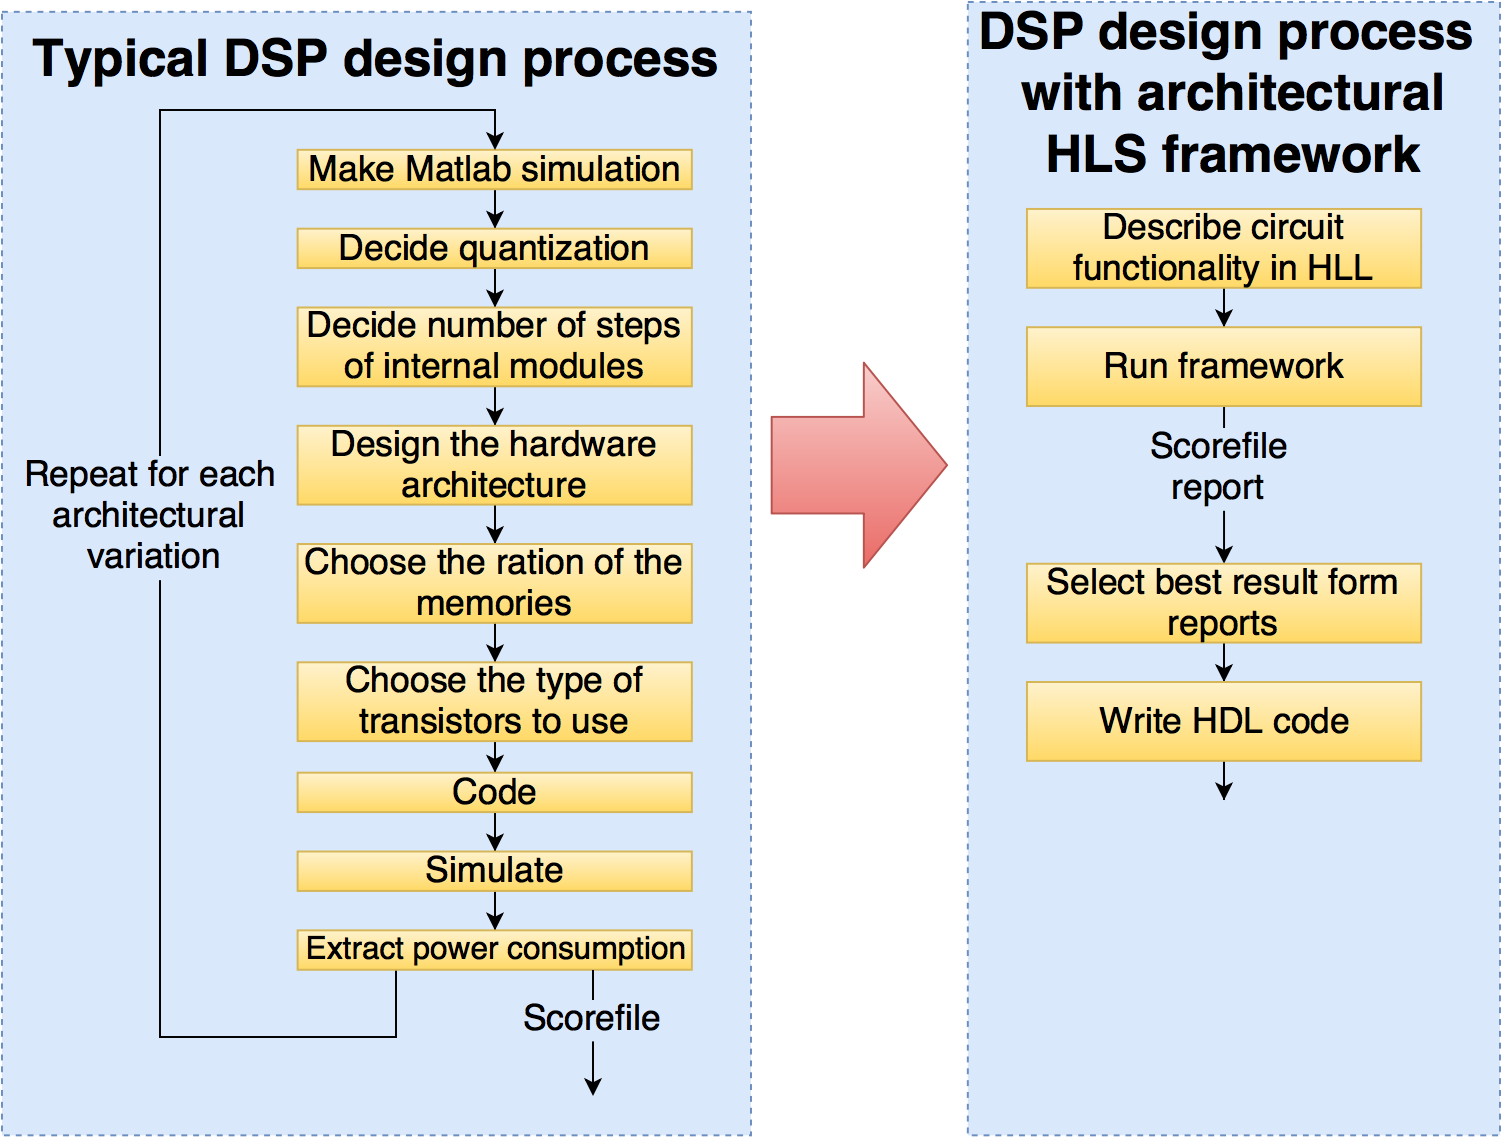
\includegraphics[width=0.75\textwidth]{../figs/Motivation.png}
\caption{\label{fig:motivationflow}Typical DSP design process compared to HLS-framework.}
\end{figure}

The thesis will look at the implementation of a framework for architectural exploration of digital hardware, targeted for \gls{asic} implementation. The ultimate goal is to create a framework that automatically explores a wide variety of architectural variations and presents the best alternatives with regards to a given design goal or constraints.
\section{Previous work}
In my specialization project \cite{holm2015pro}, conducted during the autumn of 2015, I explored the academic open source \gls{hls}-tool \textit{LegUp}. This tool has a maturity not before seen in an academic \gls{hls}-tool, and that it is open-source makes it appealing for the concept of a framework for architectural exploration of hardware. LegUp provides ANSI-C to Verilog high-level synthesis, but their focus is targeted towards implementation on \gls{fpga} architectures. The official target support of the output is limited to a few boards from the \gls{fpga} manufacturer Altera, and beta-support for a single board from Xilinx. This thesis will target \gls{asic} implementations. The findings from \cite{holm2015pro} was that there are some issues with the original version of LegUp, limiting its usability for the desired framework. The issues are mainly related to input and output of the generated modules, structure of memory management, and size of signals. A framework for architectural exploration of hardware, using \gls{hls}, was proposed in \cite{holm2015pro}. An illustration showing the tool- and information-flow of the framework is shown in \cref{fig:frameworkflow}.

\begin{figure}[hbpt]
\centering
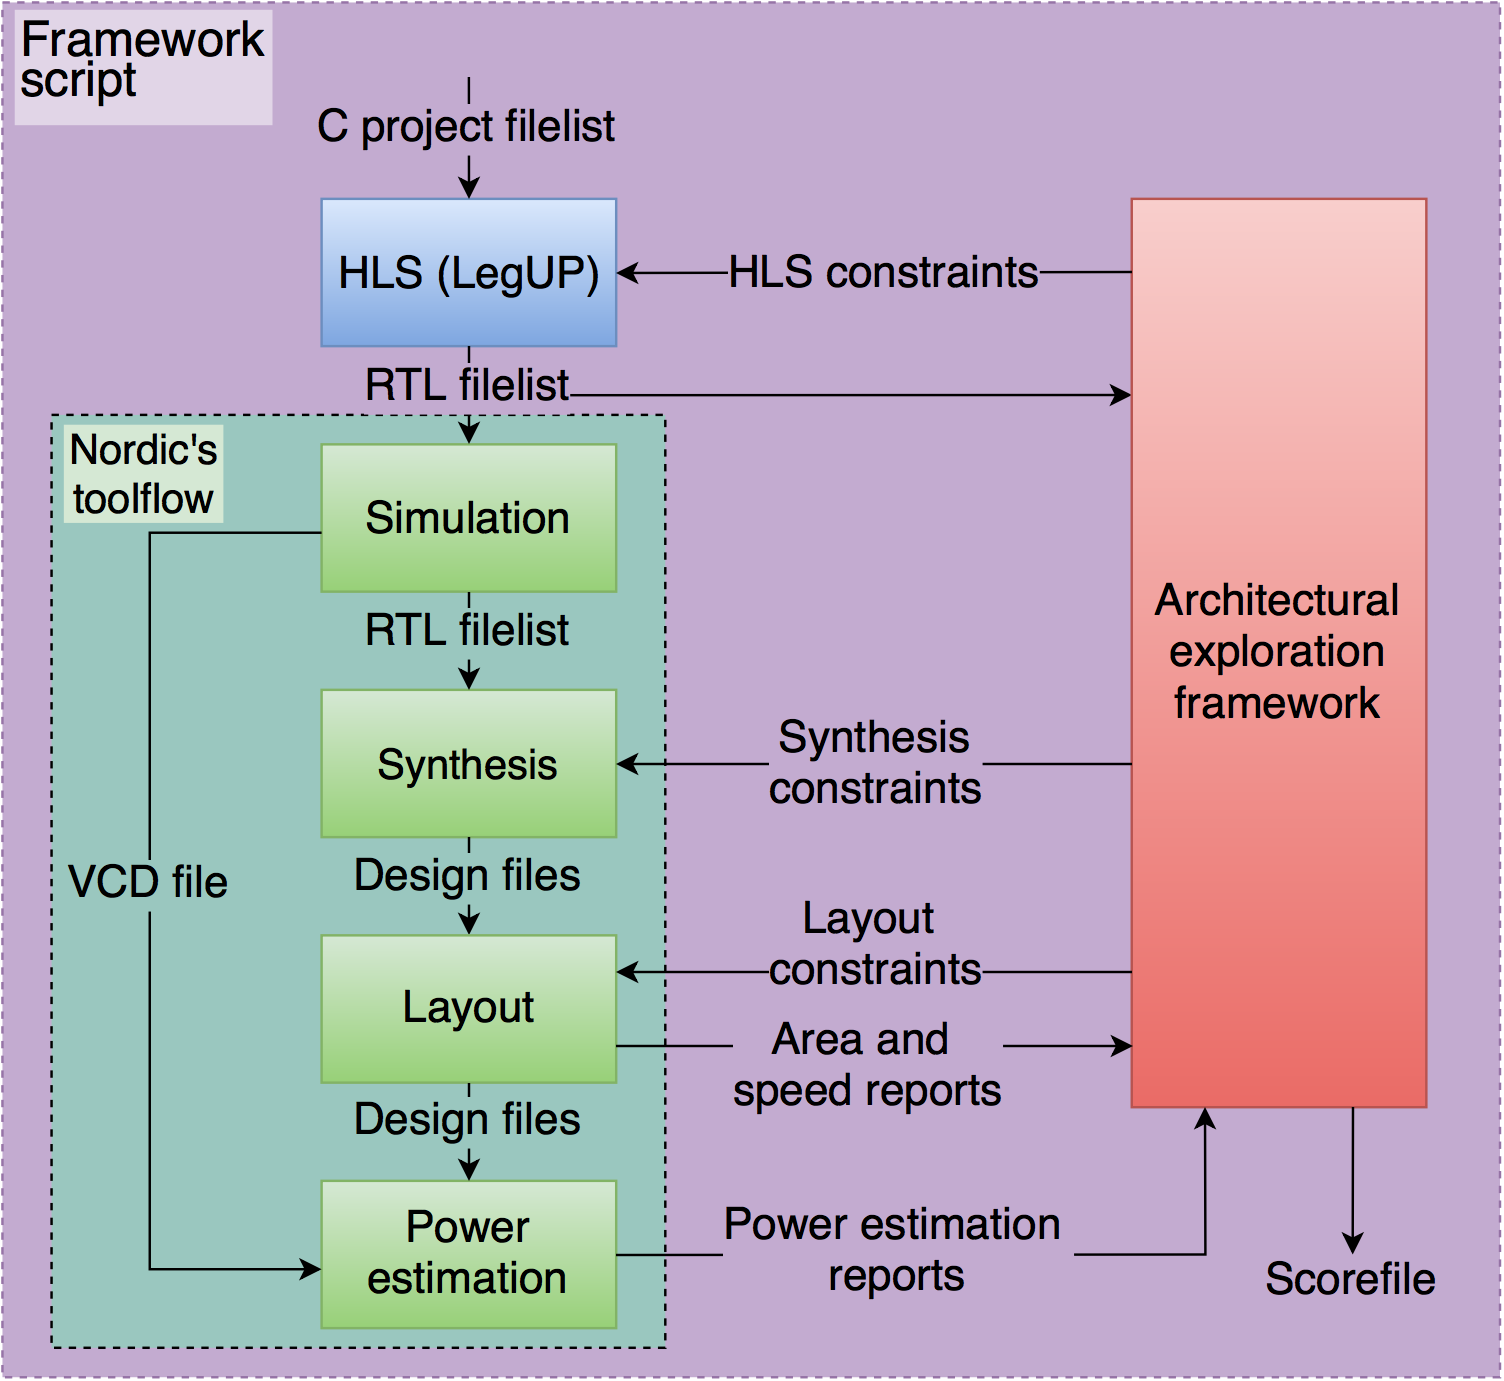
\includegraphics[width=0.75\textwidth]{../figs/Framework.png}
\caption{\label{fig:frameworkflow}Proposed framework-solution \cite{holm2015pro}.}
\end{figure}

\section{\label{sec:projectobj}Project objectives}
The initial goals of the specialization project were found to be a bit exaggerated. For this Master's thesis it was decided to focus on a smaller part of the ultimate goal, to get the necessary basics of the \gls{hls}-tool working well, before proceeding with the framework. The main goal of this thesis is therefore to resolve the issues encountered during the specialization project. It is not know if all issues can be resolved, or how time consuming it will be. Other objectives are therefore added in a prioritized order:

\newcommand\litem[1]{\item{\bfseries #1\\}}
\begin{enumerate}
\litem{Explore approaches} Two possible approaches towards resolving the issued, were described in \cite{holm2015pro}. The first step of this thesis will be to explore both these alternatives and look at positive and negative sides of each method. The outcome of this objective will affect the rest of the work with this thesis, making it an important decision. All aspects of the two approaches must therefore be taken into consideration before making a choice.
\litem{Resolve issues} For LegUp to be usable in a framework for architectural exploration, it is vital that the tool is adapted to generated Verilog suitable for \gls{asic} implementation. This objective is thought to be the most time-consuming, and its outcome is very uncertain. However, if completed successfully, the use-space of LegUp can be extended to other concepts. LegUp’s architecture is, like the input language C, quite memory-bound. \gls{ram} modules, memory controllers, and pointers are used for many things where a simple signal could have given the same result. It should be looked into if this memory-architecture can be changed by de-referencing pointers or turn memory elements into generic signals. A proper way of handling inputs and outputs should also be implemented, to avoid being limited to a certain amount of ports on the generated designs.
\litem{Create framework} When the issues have been resolved, the work with creating a framework for architectural exploration can be started. The framework will be based on the flow shown in \cref{fig:frameworkflow}, using various scripts and programs to run the tool-flow, generating constraints, and creating scorefiles. The framework should be easy to use and ideally be able to run without any interactions with the user.
\litem{Proof of concept} To verify and illustrate the concept in action, a proof of concept will be created. By creating one or more reference designs which will be run through the framework, it is expected to get a wide variety of generated designs with varying results in terms of area, power consumption, and performance. The reference design will also be implemented directly in Verilog \gls{hdl}, to compare and calculate the overhead of the \gls{hls}-generated designs.
\litem{Evaluation} Based on the results from the conducted proof of concept, a re-evaluate of LegUp's usefulness in a framework for architectural exploration of digital hardware, will be conducted. This evaluation will be based on the deviation of the results among the generated designs, as well as the overhead compared to the design written in Verilog. Other aspects can also be considered, like how well the adaption of LegUp is performed and how well the generated Verilog \gls{hdl} synthesize for \gls{asic} architectures.
\litem{Techniques for reducing overhead} The typical overhead of \gls{hls}-tools are in the range of 30-40\%. One of the initial objectives of this concept included the integration of  Nordic Semiconductor's coding style and practices, the \gls{ddvc} \cite{nordicddvc}, into LegUp's Verilog libraries. This include things like interfaces, parameters, naming conventions, power/clock domains, etc. It is assumed that this can give a large reduction of the overhead generated by the \gls{hls}-tool, when integrated into Nordic Semiconductor's existing modules.
\end{enumerate}

\section{Contributions}
The intentions of this work have been to create an adapted version of the open source \gls{hls}-tool LegUp, to make it more suited for generating Verilog targeted towards \gls{asic} architectures. It was also time to create a framework for architectural exploration of digital hardware, and to conduct a proof of concept study.

\textbf{The following list summarize the contributions made through this thesis:}
\begin{itemize}
    \item An adapted version of LegUp has been created. The adapted version support features that is important for implementation towards \gls{asic} architectures. This include the possibility of having multiple inputs and outputs in the generated modules, the inputs and outputs can be streaming, eliminating the need for stopping and starting the module for each run, and an improved method of generating testbenches that include all signals and desired testcases.
    \item A framework for architectural exploration of digital hardware has been developed. This framework can generate a large number of architectural variations with great diversity. Area, power and performance information will automatically be extracted from each design, allowing the designer to choose the best architecture for further implementation.
    \item Using a FIR-filter reference design, a proof of concept study has been conducted, showing that the framework can be used for architectural exploration of digital hardware.
    \item LegUp's usability in a framework for architectural exploration of digital hardware has been evaluated, based on results from the proof of concept study and the performance of the adapted version of LegUp.
\end{itemize}

\section{Method}
The work performed in this thesis is based on multiple research methods. Before the problem could be solved, a study of the architecture and structure of LegUp had to be conducted, to understand the connections and information-flow in the tool. This study was primarily carried out during the previous project \cite{holm2015pro}, but also continued into the work with this thesis. A plan for how to resolve each of the issues at hand was devised and discussed before being carried out, to ensure a good solution. The problems at hand requires in-depth knowledge of the libraries in LegUp, but when the source of the issue had been located, fixing the issue was based on trial and error. By replacing a piece of code with some other solution, a new output can be generated and evaluated. This process is repeated until the issue is resolved. The creation of the framework is based on the idea proposed by Isael Diaz. A study of architectural exploration and \gls{hls}-concepts had to be conducted before building the framework, to make sure the output would have the desired diversity. An experimental study of the usefulness of the created framework was conducted as a proof of concept, to check if the initial hypothesis holds. By running a reference design through the framework, a large amount of data was reported. The data was analyzed to draw the conclusion about the hypothesis.

\section{Overview of the thesis}
In general, this thesis is divided into 8 chapters, each presenting one or more of the project objectives described above, in addition to appendix. In \cref{chp:background}, the background and theory required to understand the rest of the thesis is described. Point one and two from the list above is described in \cref{chp:adaptinglegup}. Chapter \ref{chp:toolflowex} uses a design example to present a thorough description of the information-flow in LegUp and the other tools used in the framework. In \cref{chp:createframework} the third objective, the process of creating a framework, is described. The fourth objective, to create a proof of concept, is presented in \cref{chp:frameworkresults}. The evaluation of the proof of concept results, corresponding to the fifth objective, as well as a discussion of LegUp in general, with focus on its usefulness in the created framework, has been presented in \cref{chp:discussion}. Finally the work is summarized and concluded in \cref{chp:conclusion}. \Cref{chp:conclusion} also include a section of future works, describing aspects that will be interesting to look into more detail at in an eventual continuation of this project. Appendix include code-listings of designs and implementations, that are described and discussed in the main chapters.

\chapter{\label{chp:background}Theory and background}
Theory, background and previous work is important to give a thorough understanding of the material to follow in the next chapters. The base of this background chapter is written as part of the specialization project conducted during the autumn of 2015 \cite{holm2015pro}, but it is included here to allow the report to be a freestanding document. Some sections has been extended to add a deeper level of understanding to some of the described concepts than what were presented in the previous report. Some information from section 3.3 of the \textit{Methodology}-chapter has also been included in \cref{sec:toolflowbg}, as it describes part of the same tool-flow used here.

In the early days of digital hardware design, gate design and layout were performed by hand. With the rapid growth in the numbers of transistors per digital chip-design, this method quickly became too time-consuming and the need for new and more automated design methods rose. \gls{rtl}-design using \gls{hdl} has long been the standard in digital hardware design. With the increasing demand for low power and small area in large \gls{soc} designs with multiple billion transistors, this methodology is no longer sufficient if hardware manufacturers want to hit the window of opportunity with their state-of-the-art product.

\section{\label{sec:hls}High-Level Synthesis}

\gls{hls} is not a new concept as it were introduced in research papers in the late 1970s and further researched and developed in the 1980s and early 1990s \cite{martin2009high}. The available commercial \gls{hls} tools have not been providing the necessary performance and benefits over \gls{hdl} development for major hardware development companies to adapt this methodology until recently.
The concept of \gls{hls} starts with a functional specification of the circuit described using a higher abstraction level, often a \gls{hll}. A tool use target architectural model libraries and design constraints to transform this specification into hardware, represented as a \gls{rtl} or \gls{hdl}-model. The typical \gls{hls}-flow is shown in figure \ref{fig:hlsflow} and each of the transition-steps is described in the below subsections. The input libraries contain information on available hardware resources with power, area, and delay models for the target architecture.

\begin{figure}[hbpt]
\centering
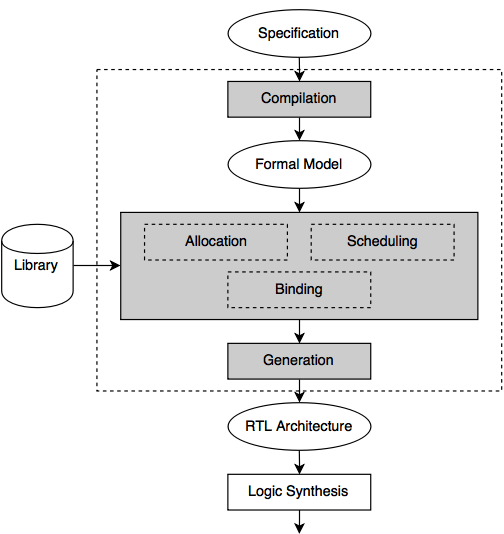
\includegraphics[width=0.55\textwidth]{../figs/HLSFlow.png}
\caption{\label{fig:hlsflow}Information flow in a typical HLS-tool \cite{coussy2009introduction}.}
\end{figure}

\subsubsection{Compilation}

The first step of \gls{hls} is to compile the functional specification into a formal model. This model can vary between different tools, and can be either a specific representation language or a graphic representation of the flow. The formal model is decided by the developers of the \gls{hls} tool. 

\subsubsection{Allocation}

Necessary hardware resources, such as functional units, storage-, and connectivity-components needs to be selected from a given \gls{rtl} component library in order to satisfy the specification and design constraints. Some \gls{hls} tools can also add more resources in the scheduling and binding tasks, if this is needed to meet given constraints.

\subsubsection{Scheduling}
Scheduling arranges all operations in an optimized sequence so that variables are read from sources and brought to the input of the correct functional unit for execution and to the destination afterwards. The scheduler takes all dependencies into account when scheduling the operations, in order to get the most efficient result, as some operations can be executed in parallel if no dependencies exist and there is available resources. Operations can be scheduled to finish in one, or take multiple clock-cycles, and operations can also be chained to eliminate the need for storing the result between operations, and to reduce the total number of cycles needed. 
\subsubsection{Binding}
In the binding task, all clock-cycle-crossing variables, operations, and transfers are bound to a free resource, in the time-frame when it is scheduled. Non-overlapping or mutually exclusive variables can be bound to the the same storage unit, and operations can be bound to the best optimized functional unit if multiple alternatives are available. Each transfer from component to component, either storage or functional unit, needs to be bound to a connection unit, such as a bus or a multiplexer.
\subsubsection{RTL Generation}
The generated \gls{rtl} usually consists of two parts, a control-unit and a data-path-unit. The control-unit is often implemented as a \gls{fsm}, which set control-signals to the data-path, and controls the current and next-state of the system. The data-path contains storage-, functional-, and connection-units. An example of this division is shown in \cref{fig:hlsrtl}.
\begin{figure}[hbpt]
\centering
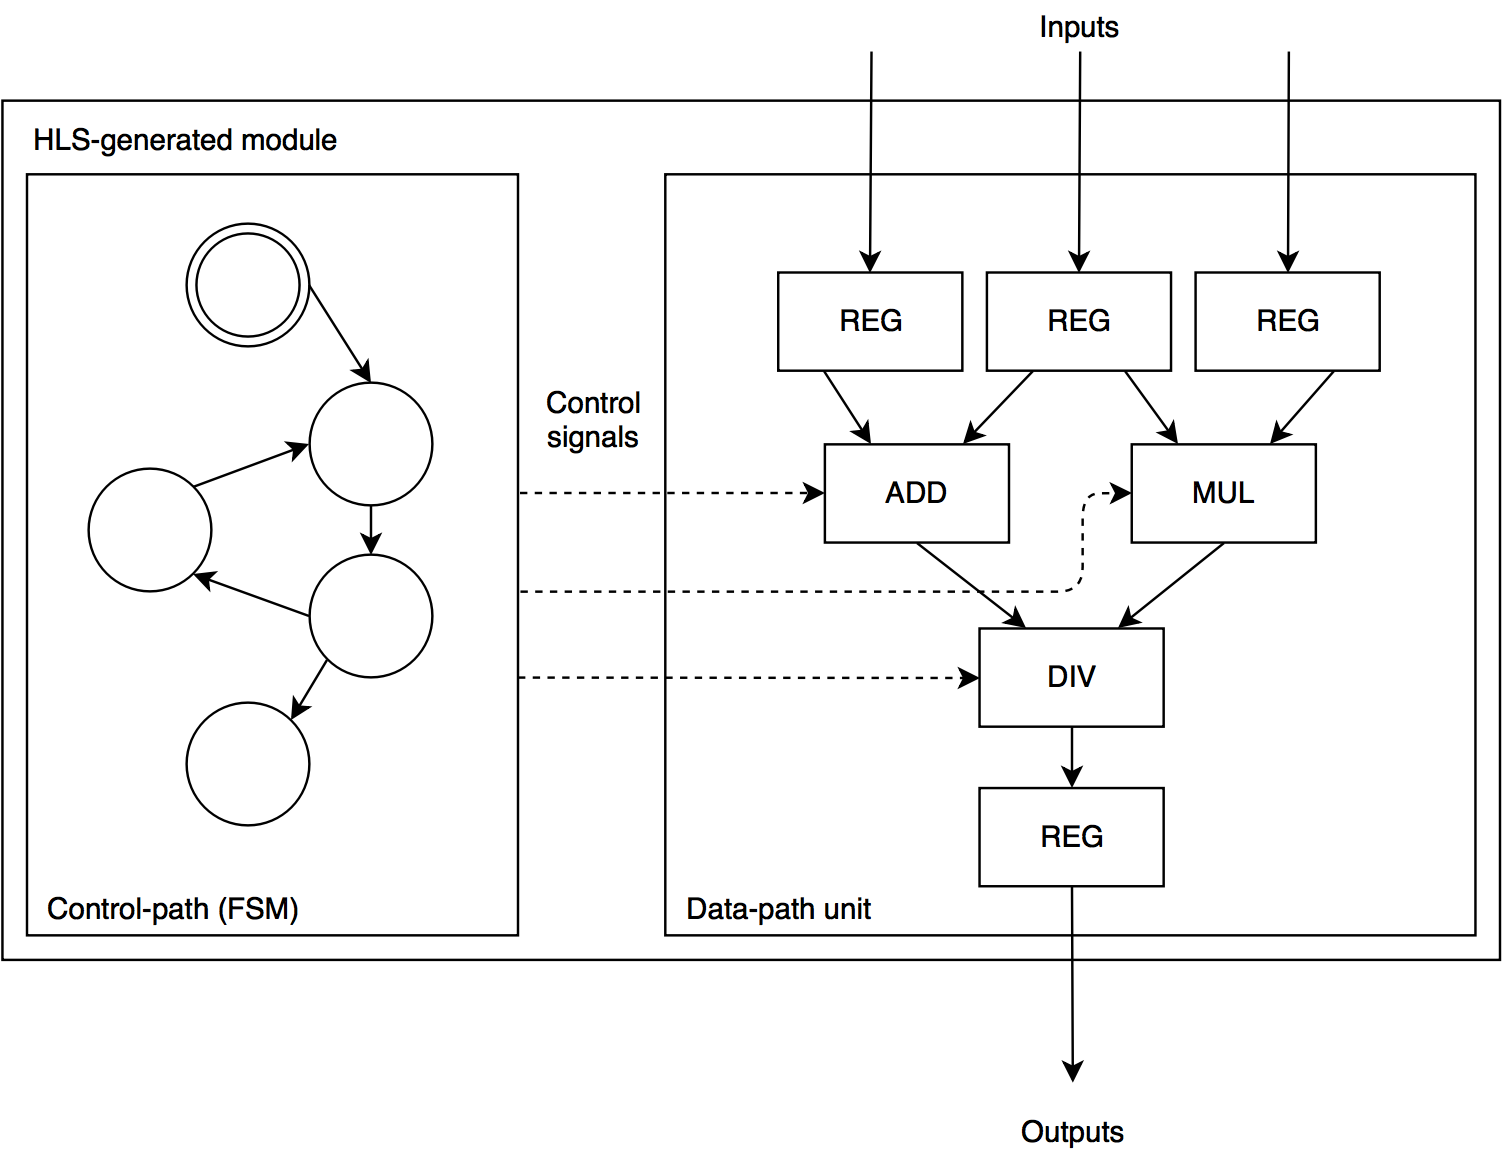
\includegraphics[width=0.65\textwidth]{../figs/HLSRTL.png}
\caption{\label{fig:hlsrtl}Typical division of control and data-path in the generated \gls{rtl} from \gls{hls}.}
\end{figure}
Depending on the intensiveness of the binding step, the output \gls{rtl} can be tightly or loosely bound to the available resources. If an operation is not bound to a specific unit, it is up to the following logic synthesis of the \gls{rtl} to bind the operations to available resources. The different types of \gls{rtl} output are illustrated by the following example. \textit{a = b * c} executing in state \textit{n}:

\begin{minipage}[t][300px]{\textwidth}
\textbf{Without any binding:}%\hfill\vspace{-\baselineskip}
\begin{verbatim}
state (n): a = b * c;
go to state (n + 1);
\end{verbatim}
\textbf{With storage binding:}%\hfill\vspace{-\baselineskip}
\begin{verbatim}
state (n): S(1) = S(2) * S(3);
go to state (n + 1);
\end{verbatim}
\textbf{With functional-unit binding:}%\hfill\vspace{-\baselineskip}
\begin{verbatim}
state (n): a = MUL1 (b, c);
go to state (n + 1);
\end{verbatim}
\textbf{With storage and functional-unit binding:}%\hfill\vspace{-\baselineskip}
\begin{verbatim}
state (n): S(1)=MUL1 (S(2), S(3));
go to state (n + 1);
\end{verbatim}
\textbf{With storage, functional-unit, and connectivity binding:}%\hfill\vspace{-\baselineskip}
\begin{verbatim}
state (n): BUS1 = S(2); BUS2 = S(3);
BUS3 = MUL1 (BUS1, BUS2);
S(1) = BUS3;
go to state (n + 1);
\end{verbatim}
\end{minipage}

A loosely bound \gls{rtl} gives the synthesis-tool the flexibility to optimize the unit binding to updated timing estimates, delays, and loads given by the layout and floor-planning tools.

\section{LegUp}
The \gls{hls} tool used in this project is called LegUp \cite{canis2011legup}. LegUp is an open-source academic tool developed at the University of Toronto, Canada. LegUp's goal is to \textit{"allow researchers to experiment with new \gls{hls} algorithms without building a new infrastructure from scratch"} and their long-term vision is to \textit{"make \gls{fpga} programming easier for software developers"}. LegUp takes \gls{ansi}-C as input and generates synthesizable Verilog \gls{hdl} as output. The developers of LegUp have primarily focused on support for a variety of \gls{fpga} boards from manufacturer Altera, but in the latest version (4.0), beta support for Xilinx devices and possibility to configure the tool to generate generic Verilog to target other \gls{fpga} vendors or even \gls{asic} through use of generic dividers, has been introduced. The big advantage of LegUp compared to similar, commercial tools, is that it is open-source and therefore can be configured to target different architectures. The \gls{rtl} and \gls{hdl} generating part of the tool can be modified or replaced to fit the programmers needs.
Since LegUp, in its unmodified form, target \gls{fpga} devices, it support three different synthesis flows; pure-\gls{sw}, hybrid, and pure-\gls{hw}. The two first synthesis flows will implement a TigerMIPS \cite{tigmips} soft processor, which will run part of the C code. The partitioning of \gls{sw} and \gls{hw} in the individual modules are described in \cref{tab:legupflows}. It is the pure-\gls{hw} flow that will be the focus of this project.

\begin{table}[hbpt]
    \centering
    \caption{\label{tab:legupflows}HLS-flows supported by LegUp and partitioning between SW and HW}
    \begin{tabular}{lp{4.8cm}p{4.8cm}}
      \textbf{Flow} & \textbf{Functions run in hardware} & \textbf{Functions run in software}\\
      \toprule
      Pure-SW & None & All \\
      \hline
      Hybrid & Specified hardware-accelerated functions & All other functions \\
      \hline
      Pure-HW & All & None\\
      \bottomrule
    \end{tabular}
\end{table}

\subsection{Producing Verilog Output}
LegUp is made up of two components; a frontend pass and a target backend pass to the LLVM compiler infrastructure. 
The information flow in LegUp, shown in figure \ref{fig:legupflow}, follows the same principle as the information flow described in section \ref{sec:hls}.
\begin{figure}[hbpt]
\centering
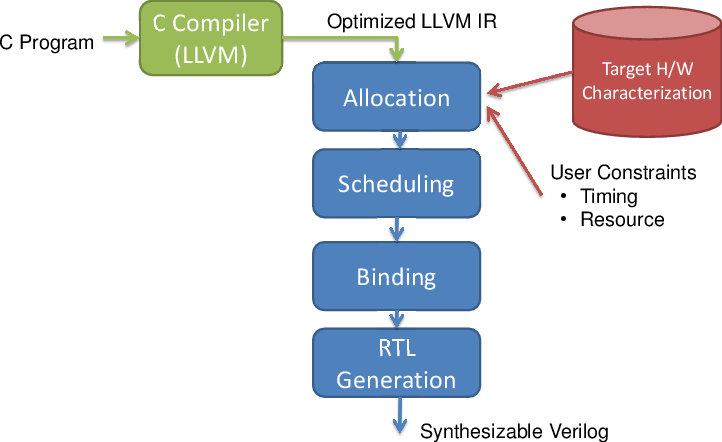
\includegraphics[width=0.6\textwidth]{../figs/LegUpFlow.png}
\caption{\label{fig:legupflow}Information flow in LegUp \cite{legupmaual}.}
\end{figure}
The LegUp LLVM frontend takes LLVM-\gls{ir} compiled by clang, a C frontend for LLVM, as input and links in custom written functions like memcpy, memset and memmove, which do not exist in hardware, but that LLVM assumes exist in the C library. 
The LegUp backend pass performs allocation, scheduling and binding as described in section \ref{sec:hls}. In the next step, \gls{rtl}-module objects that represents the final hardware circuit are generated from each LLVM instruction. Ultimately, Verilog code corresponding to each of the \gls{rtl}-modules is output to a file.

The allocation, scheduling, and binding in LegUp is performed based on information about available resources and timing information about the specified target FPGA-board, in addition to user-defined constraints and setting. The available information about the FPGA-boards allows for precise scheduling and binding to the available resources. Since the implementation of ASIC designs are quite different from the architecture and implementation of designs on FPGAs, the resource and timing information will not be as easily obtained for the target architecture. 

\subsection{\label{sec:legupclasses}Classes}
LegUp has some predefined classes that is important for the understanding of the description of how LegUp is adapted for generating more ASIC compliant Verilog. The following subsections will describe these classes in more detail.
\subsubsection{RTLModule}
The RTLModule class models a hardware RTL module. The class stores information about all ports (inputs and outputs), signals, parameters and sub-modules. Each function declared in the C-code transforms into a RTLModule object. Each function that is called from the function will be added as a sub-module to the RTLModule object, meaning a module instantiation will be added to the module. Important member functions in the RTLModule class is:
\begin{compactdesc}
    \item[getName()] \hfill \\
    Returns a string containing the name of the RTLModule, i.e. "main" for the module generated by the main-function in the C-program.
    \item[find(std::string signal)] \hfill \\
    Takes a string containing a signal name as parameter and returns a pointer to the RTLSignal in the RTLModule with that name.
    \item[addParam()] \hfill \\
    Adds a parameter to the module. The function returns a pointer to the generated RTLSignal object.
    \item[addIn()] \hfill \\
    Adds an input port to the module. The function returns a pointer to the generated RTLSignal object.
    \item[addOut()] \hfill \\
    Adds an output port to the module. The function returns a pointer to the generated RTLSignal object.
    \item[addRegOut()] \hfill \\
    Adds a registered output port to the module. The function returns a pointer to the generated RTLSignal object.
    \item[addReg()] \hfill \\
    Adds a register signal to the module. The function returns a pointer to the generated RTLSignal object.
    \item[addWire()] \hfill \\
    Adds a wire signal to the module. The function returns a pointer to the generated RTLSignal object.
    \item[addModule()] \hfill \\
    Adds a instantiation of another module to the module. The function returns a pointer to the generated RTLModule
    object.
\end{compactdesc}
\subsubsection{RTLSignal}
The RTLSignal class represents the signals within an RTLModule. Both internal signals, port signals and condition signals are all modelled usign the RTLSignal class. Important member functions of the class is:
\begin{compactdesc}
    \item[getName()] \hfill \\
    Returns a string containing the name of the RTLSignal, i.e. "clk" for the clock signal.
    \item[getType()] \hfill \\
    Returns a string describing the signal type. The type can be reg, wire, input, output and output reg.
    \item[getNumDrivers()] \hfill \\
    Return the number of driving RTLSignals. 
    \item[getDriver(unsigned i)] \hfill \\
    Returns a pointer to the i-th driving RTLSignal.
    \item[getCondition(unsigned i)] \hfill \\
    Returns a pointer to the condition signal of the i-th driving RTLSignal.
    \item[addCondition(RTLSignal *cond, RTLSignal *driver)] \hfill \\
    Adds a conditional driver. If the RTLSignal \textit{cond} is true, the RTLSignal \textit{driver} drives the signal. 
    \item[connect(RTLSignal *s)] \hfill \\
    Connect this signal unconditionally to another RTLSignal.
    \item[getWidth()] \hfill \\
    Returns a pointer to a RTLWidth object, describing the width of the RTLSignal.
    \item[isOp()] \hfill \\
    Returns true if the RTLSignal is an RTLOp object.
\end{compactdesc}
\subsubsection{RTLOp}
The RTLOp class is a subclass of the RTLSignal class, representing an operation with one, two or three operands. Each operand is a RTLSignal. The operation can be an arithmetic operation like addition, subtraction, multiplication, or division, and it can also be logical operations like AND, OR, and XOR, or even comparison operations like equal, not equal, less than, less than or equal, greater than, and greater than or equal. The whole list can be seen in the class reference \cite{rtlopclassref}. A RTLOp object modelleing an AND operation of two operands, operand1 and operand2, will in Verilog correspond to the operation \verb!operand1 & operand2!. Some important member functions are:
\begin{compactdesc}
    \item[getOperand(int i)] \hfill \\
    Returns a pointer to i-th operand of the RTLOp object.
    \item[getNumOperands()] \hfill \\
    Returns the number of operands of the RTLOp object.
    \item[setOperand(int i, RTLSignal *s)] \hfill \\
    Sets the i-th operand to the RTLSignal \textit{s}.
\end{compactdesc}
\subsubsection{RTLWidth}
The RTLWidth class represents the bitwidth of a RTLSignal. An RTLWidth is defined by high and low bits, for instance 31,0 for a 32 bit signal. This will transform into \verb![31:0]! in Verilog.
\subsubsection{RAM}
The RAM class models RAM modules in LegUp. Whenever a variable is loaded or stored, a RAM module is generated to handle the loads and stores. The RAM objects can be divided into two scopes; LOCAL and GLOBAL. A Local RAM object is local to a given function and cannot be accessed from other functions. A global RAM object will be implemented in a global memory controller, and all modules that use the variable can connect to the RAM via the memory controller. Some important member functions are:
\begin{compactdesc}
    \item[getName()] \hfill \\
    Returns a string containing the name of the RAM module, i.e. "main\_0\_1" for the RAM module generated for the first parameter to the main function declared as volatile (output parameters) in the C-code.
    \item[isROM()] \hfill \\
    Returns true if the RAM is read-only.
    \item[getScope()] \hfill \\
    Returns if the RAM is in the local or global scope.
\end{compactdesc}


\subsection{Constraints}
Constraints is a important part of LegUp and its usage in this project. The constraints are used for setting design goals and limitations on design, and to specify how the \gls{hls}-flow shall be executed. All available constraints are described in the constraint manual \cite{legupconst}, but the ones used in this project are described in \cref{tab:constraintssescription}. Constraints play an important role in this concept, as the idea is to generate multiple designs that can be compared in terms of area and power consumption. For the designs to be different, varying constraints are used for generating the designs. Some constraints are considered \textit{required}, as they must be set for the generated design to be compatible with the tool-flow. HLS constraints are used for getting different Verilog output from LegUp. Other constraints from the constraint manual can be also be used, but these were selected for this project as their description signalize possibility to affecting the output.
\begin{table}[hbtp]
    \centering
    \begin{tabular}{l|p{6.4cm}|c}
    \multicolumn{3}{c}{\textbf{Required constraints}} \\
    \toprule
    \multicolumn{1}{c}{\textbf{Parameter name}} & \multicolumn{1}{c}{\textbf{Description}} & \specialcell{\textbf{Required}\\\textbf{value}} \\
    \midrule
    \small{DIVIDER\_MODULE} & Use generic divider module rather than Altera primitive & \textit{generic} \\
    \hline
    \specialcelll{\small{EXPLICIT\_}\\\small{LPM\_MULTS}} & Use Altera primitive multiplier rather than Verilog multiply operator (*) & \textit{0} \\
    \hline
    \small{INFERRED\_RAMS} & Use Verilog inferred RAMs rather than Altera altsyncram modules & \textit{1} \\
    \hline
    \specialcelll[t]{\small{INFERRED\_}\\\small{RAM\_FORMAT}} & Select format of inferred RAMs. Altera: multiple always blocks, Xilinx: same always block & \textit{xilinx} \\
    \hline
    \small{LOCAL\_RAMS} & Infer all RAMs as local RAMs rather than global RAMs. RAMs being accessed by multiple functions will override this setting & \textit{1} \\
    \hline
    \small{VSIM\_NO\_ASSERT} & Disable triple-equality assertions. This causes simulation to fail & \textit{1} \\
    \midrule
    \multicolumn{3}{c}{\textbf{HLS constraints}} \\
    \toprule
    \multicolumn{1}{c}{\textbf{Parameter name}} & \multicolumn{2}{c}{\textbf{Description}} \\
    \midrule
    \small{SDC\_NO\_CHAINING} & \multicolumn{2}{p{8cm}}{Schedule each operations into a separate clock cycle} \\
    \hline
    \small{MB\_MINIMIZE\_HW} & \multicolumn{2}{p{8cm}}{Run LegUp-pass that tries to minimize signal sizes} \\
    \hline
    \small{CASE\_FSM} & \multicolumn{2}{p{8cm}}{Use case-statements in FSM rather than If-Else} \\
    \hline
    \small{PIPELINE\_ALL} & \multicolumn{2}{p{8cm}}{Enable pipelining for all loops, regardless of loop-label} \\
    \hline
    \specialcelll{\small{ENABLE\_}\\\small{PATTERN\_SHARING}} & \multicolumn{2}{p{8cm}}{Turn on resource sharing for patterns in \gls{dfg}} \\
    \hline
    \specialcelll{\small{DUAL\_PORT\_}\\\small{BINDING}} & \multicolumn{2}{p{8cm}}{Use dual-ported on-chip memories} \\
    \bottomrule
    \end{tabular}
    \caption{Descriptions of constraints used in this project}
    \label{tab:constraintssescription}
\end{table}

\section{\label{sec:LLVM}LLVM}
LLVM \cite{LLVM:CGO04}, formerly Low-Level Virtual Machine, is a compiler framework that was originally developed as a research infrastructure to investigate dynamic compilation techniques for static and dynamic programming languages, at the University of Illinois in 2000. It is now a open-source project with many contributors from both industry, research groups and individuals, and it is used by companies like Apple in their Xcode \gls{ide} \cite{llvmapple} and Sony for their PS4 developer toolchain \cite{llvmsony}. LLVM support a large number of frontends for programming languages, including Clang \cite{clang} which support C, C++, Obcjective-C, and Objective-C++, and is compatible with \gls{gcc}. It also supports a large number of backend target architectures. Figure \ref{fig:llvmcompiler} shows how different source languages can be input to the frontend compilers of LLVM, which translate the source into an \gls{ir}. The \gls{ir} is then optimized using LLVM's optimizer. At this stage, different source languages can be linked together, and even object files compiled using standard \gls{gcc} can be linked at this stage. The optimized \gls{ir} is then translated into the target architecture by the backend.

\begin{figure}[hbpt]
\centering
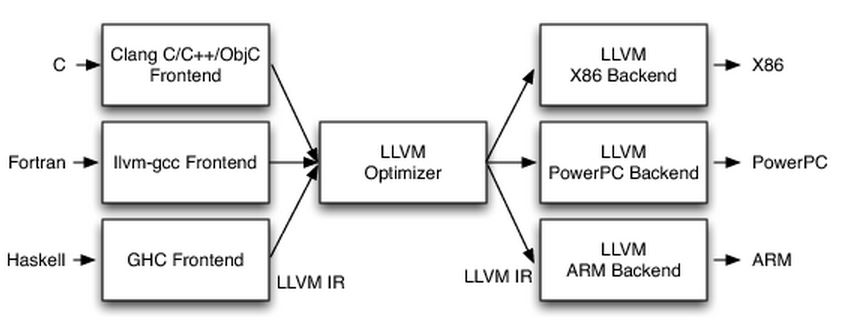
\includegraphics[width=\textwidth]{../figs/LLVMCompiler.jpg}
\caption{\label{fig:llvmcompiler}LLVM's three-phase compiler structure \cite{llvmarch}.}
\end{figure}

\subsection{Intermediate Representation}
LLVM use a human readable assembly-like, strongly typed RISC instruction set as their \gls{ir}, with support for an infinite number of temporary registers of the form \%0, \%1, etc. LLVM-\gls{ir} can also output a dense bitcode format for serialization. Conversion between the bitcode-format and the human-readable format, and vice versa, can be done with the commands "\verb!llvm-dis!" and "\verb!llvm-as!", for dis-assembly and assembly.

Some parts of the LLVM \gls{ir} will be described in \cref{chp:toolflowex}. The whole language are too large to be fully explained here, but interested readers can read more about the syntax in the \textit{LLVM Language Reference Manual} \cite{llvmlangman}.

\section{Alternative hardware design methods}
\gls{hls} is not the only alternative to \gls{hdl}-languages, if you want to design digital hardware at a higher level of abstraction. The following subsections will shortly describe two alternative approaches to digital hardware design. 
\subsection{Chisel}
One interesting approach to designing hardware with a higher level of abstraction, is the Chisel \gls{hcl} \cite{bachrach2012chisel}, developed at UC Berkeley. Unlike \gls{hdl} languages like VHDL and Verilog, which were originally designed as simulation languages and later adopted as a basic for synthesis, Chisel was created as a \gls{hcl} and is thus \textit{synthesizable by construction}. This entails that no conversion from C, or other \gls{hll}, into gates is performed, only generation of generic low-level Verilog with no overhead. Chisel is a \gls{dsl} built on Scala \cite{odersky2004overview} with its own syntax, but Scala syntax can also be used to get even greater abstraction in your design. A big advantage using Chisel is its high simulation speed, using C++-based cycle-accurate software simulators.

\subsection{Functional programming}
Functional programming is a relatively different method of hardware design, as it consists only of mathematical functions and immutable data. Two examples of hardware design using functional programming is C$\lambda$aSH \cite{baaij2009clash} and Lava \cite{bjesse1998lava}. Both Lava and C$\lambda$ash are compilers for the functional programming language Haskell \cite{haskellonline}, but while Lava is an embedded \gls{dsl} like Chisel, with its own syntax, C$\lambda$ash use Haskell syntax and semantics, and use a static analysis approach towards synthesis.

\section{Programming concepts}
In high-level programming languages like C and C++ and in \gls{hdl} languages like Verilog, the use of programming concepts are extensively used. This section describes some concepts that are frequently referred throughout this report.
\subsection{Structures}
A structure, or struct for short, is a complex data-type that can contain multiple other variables of different data-types. 
\subsection{Classes}
A class can contain multiple variables of different data-types, like a struct, but in addition a class can have member.functions and divide its member into a public and a private scope. The private members of a class can only be accessed through public member-functions. This added level of security increase the level of integrity of the objects.
\subsection{Pointers}
A pointer is a variable that is defined to point at a location in memory where another object is stores. The pointer itself contains the memory address of the object it points at.
\subsection{Declaration}
Declaration refers to the process of declaring a type or an object that will be used at a later stage. This can for instance be be a struct in C, a class in C++ or a module in Verilog. A type or an object, needs only to be declared once and can then be used as many times as necessary. An example of a declaration of a struct in C: 
\lstset{language=C++, style=Cstyle}
\begin{lstlisting}
struct Book { char title[128], 
              char author[128], 
              int isbn 
            } ;
\end{lstlisting}
\subsection{Instantiation}
Instantiation is when the object you created with your declaration, is created and stored at a designated location in memory. When you instantiate an object, you usually assigns it a variable, or name, that you use throughout the scope of the object to reference the object. In Verilog we often talk about module \textit{instantiation}. This is the same concept as in \gls{hll}-languages, but here a declared module is placed inside another module, making it a \textit{sub-module}.
\subsection{Assignment}
Assignment is when you give an instantiated object a value, i.e. you are assigning a value to the object.
\subsection{Defining types}
A user-defined structure or object can be defined as a type in C. The struct-example from above can be defined as a type by the line:
\begin{lstlisting}
typedef struct Book Book_t
\end{lstlisting}
Now an object of the type \textit{struct Book} can be instantiated using the line:

\verb!Book_t mybook!,

where \textit{mybook} is the variable name. Using \textit{typedef} saves time and reduce code-size in many cases.

\section{\label{sec:powdiss}Power dissipation in CMOS circuits}
The power dissipation in CMOS circuits can be divided into three categories \cite{panda2010power}, \textit{dynamic power}, \textit{short-circuit power} and \textit{leakage power}. This gives a total power dissipation of:
\begin{equation}
    P_{total} = P_{dynamic} + P_{short-circuit} + P_{leakage}
\end{equation}

Figure \cref{fig:powerdisscmos} shows the distribution of the power components of the CMOS circuit. Each component is described in more detail in the following subsections, where \textit{switching power} corresponds to $P_{dynamic}$, \textit{internal power} corresponds to $P_{short-curcuit}$, and \textit{leakage power} to $P_{leakage}$.
\begin{figure}[hbpt]
\centering
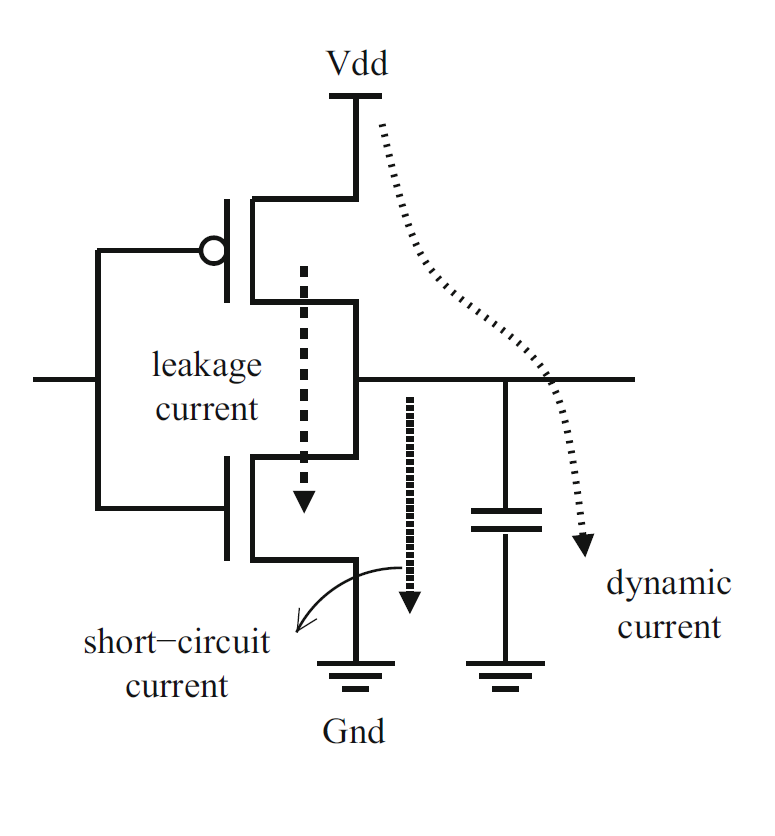
\includegraphics[width=0.4\textwidth]{../figs/PowerDissipation.png}
\caption{\label{fig:powerdisscmos}Power dissipation components distribution \cite{panda2010power}.}
\end{figure}

\subsection{Switching power}
\textit{Switching power} arise whenever a signal change the logic state from 0 to 1, causing the load capacitance to be charged by the power supply. Half the energy drawn from the power supply needed to charge the capacitance, is dissipated as heat in the process. The \textit{switching power} depends on the frequency of the switching, the switching factor of gates and the load capacitance in addition to the supply voltage. 

\subsection{Internal power}
The \textit{internal power} is the power used to charge and discharge the internal capacitance of the circuits whenever a pin change its state. A large part of the \textit{internal power} is the short-circuit power. In the short time when both the pMOS and nMOS transistor of the CMOS circuit is \textit{on}, a current will be drawn from the source $V_{dd}$ to ground through the short-circuit that will occur. 

\subsection{Leakage power}
Whenever the circuits are turned \textit{on}, a small leakage current will be drawn from the gates. The leakage power is mostly caused by sub-threshold currents and reverse biased diodes in the circuits. The leakage current increase when the technology shrinks, making leakage a bigger problem today than before. 

\section{\label{sec:toolflowbg}Tool-flow}
This tool-flow section will describe all the tools that are used throughout this thesis, and the connection and data-flow between the different tools. This flow is based on the standard tool-flow used at Nordic Semiconductor, as well as some parts adapted from the "\textit{automated area and power estimation tool-flow}" created by Joar Talstad for his Master thesis \cite{talstad15master}. Most of the tool-flow is based on scripts and Makefiles that can be run from a Linux shell, but there are also some GUI-tools available that will be mentioned briefly in \cref{chp:toolflowex}. The following subsection will describe the different sections of the tool-flow in detail. The flow in LegUp will not be described here, as this is covered above and will be presented in more detail in \cref{chp:toolflowex}.

\subsection{Simulation}
Simulation is run to verify the correctness of a design and to help detect and eliminate potential bugs. In this project, the simulation tool also generates a \gls{vcd}-file, showing switching activity during simulation. This file is used in the power analysis tool later in the flow, to get a realistic input of the amount of switching in the design. Simulation is performed using the tool ModelSim for Questa-64, version 10.2b 2013.05 \cite{questasim}. Simulation is executed by calling the script \textit{RUN\_ALL}. The \gls{rtl}-design filelist and a file containing a testbench module must be specified in the filelist found in the \textit{sim/tb/}-directory, at this is used as input to the simulation tool.
\subsection{Synthesis}
Synthesis translates a \gls{rtl}-design written in a \gls{hdl}-language, like Verilog or VHDL, into a netlist for a specified target library. The tool used for synthesis in this project is Synopsys Design Compiler, version I-2013.12-SP2 \cite{syndescomp}. A cell library describing 180nm technology is used as the target architecture. A Makefile is used to start synthesis, and the command \verb!make compile! runs the full synthesis. The netlist generated by synthesis is found in the file \textit{designName.mapped.v} in the \textit{result}-directory. This netlist is used as input for the layout-tool. Synthesis generated reports showing area-estimates, register count, critical path and static power estimates for the design. As the design will be processed further through the tool-flow, these reports are not that accurate or useful.
\subsection{Layout}
Layout translates the netlist generated during synthesis into a chip layout. The tool used for layout in this project is Synopsys IC Compiler, version L-2016.03-SP1 \cite{syniccomp}. A Makefile is used to start layout, and the command \verb!make outputs_cts! runs the correct layout-script. Layout produces a new netlist-file, stored in the file \textit{designName.output.v} in the \textit{result}-directory. This netlist is used in the power analysis tool for estimating power consumption. From layout, reports about area and critical paths are stored in the \textit{reports}-directory. These results are more accurate, as they were gathered from the actual chip layout.
\subsection{\label{sec:powest}Power analysis}
Power analysss is performed to get an early indication on how much power the final design will be consuming. The tool used power analysis in this project is Synopsys Primetime, version K-2015.12-SP3. To get accurate power estimates, the switching activity file generated during simulating is used together with the netlist output from layout. The conclusion from \cite{talstad15master} were that this method is well suited for making RTL-design trade-offs based on power consumption in multi-voltage designs, providing accurate results. Power analysis is run on five different power scenarios, each giving a separate result for each of the three power dissipation categories described in \cref{sec:powdiss}. The reports are stored in the \textit{reports}-directory.

\section{Linux tools}
Some tools available in Linux is used throughout the scripts created in this thesis. The following subsections will give a short introduction to the most important tools and its usage.
\subsection{bash}
\textit{bash} is the default shell, or command language interpreter, in Linux. A shell processes macros and executes commands. By adding commands to a file, i.e. a script, a long list of commands can be executed in order. For a script to be executed in the bash shell, the \textit{shebang}-line, the first line of the file, needs to contain the path to the bash shell. The line \verb!#!/bin/bash! can be used in most cases, but for portability, the line \verb!#!/usr/bin/env bash! is the safest choice.

\subsection{make}
\textit{make} is a tool used to decide which parts of a large program needs to be recompiled. The synopsis of \textit{make} is:

\verb!make [OPTIONS] [TARGETS]!

Some options for make are:\\
\verb!-f MAKEFILE     !\textit{Provide the path to the Makefile}
\verb

To use \textit{make}, a \textit{Makefile} describing the relationships between the files of the program is needed. If the Makefile is present in the folder where you run the \textit{make}-tool, you do not need to specify the path to the file. The Makefile can define multiple targets, each performing a separate compilation. There can be dependencies between the targets, forcing the dependency-targets to be compiled before specified target.
\subsection{grep}
\textit{grep} is used to search for the occurrence of a pattern in a given file, and print each line found. The synopsis of \textit{grep} is:

\verb!grep [OPTIONS] PATTERN [FILE...]!

where PATTERN is the pattern to be matched, and FILE is the path to the file(s) to be searched.

Some important options used with \textit{grep} are:\\
\verb!-e PATTERN      !\textit{Provide multiple patterns}\\
\verb!-f FILE         !\textit{Get PATTERN from file}\\
\verb!-c              !\textit{Return number of matched lines}\\
\verb!-m NUM          !\textit{Exit after NUM matches}

If you run the command "\verb!grep "one"!" on a file containing the following lines:

\verb!one two three!\\
\verb!one!\\
\verb!two!

the output will be:

\verb!one two three!\\
\verb!two!

as the first and the last line of the input contains the pattern \textit{two}.

\subsection{Substring replacement}

As \textit{grep} returns the whole line that were matched we need a way to eliminate unwanted information from the returned line. For this purpose, the tool \textit{sed} could be used, but when using the \textit{bash}-shell for scripts, a similar tool called substring replacement is included natively. The syntax of substring replacement is:

\verb!\${string/substring/replacement}!

where \textit{string} is a string, \textit{substring} is the text to be replaced and \textit{replacement} is the string that \textit{substring} will be replaced with. Notice that \textit{string} can be both a literate string and a variable containing a string, depending on the use. This format will only replace the first occurrence of \textit{substring} on each line of \textit{string}. To replace all occurrences, this format must be used:

\verb!\${string//substring/replacement}!

If the command "\verb!${"one two one two"//one/three}!" is run, the output would give \verb!"three two three two"!, as all occurrences of the substring \textit{one} will be replaced by \textit{three}.

\section{Reference design}
\label{sec:refdes}
This thesis will look into whether or not LegUp can be used as the HLS-tool in a framework for architectural exploration of hardware. In order to get some output from LegUp than can be compared towards each other, a reference design must be created. The design must be something that can be implemented both in C and Verilog and it should be easy to implement. In \cite{holm2015pro}, two reference designs were implemented; a FIR-filter and a SAP-1 architecture. The FIR-filter will be used as the reference design in this project, as this is a regular structure that easily can be implemented and verified. The SAP-1 architecture would have been a interesting second reference design, as it consists of a FSM, just like the output from LegUp. Unfortunately, this architecture has too many design-parts that makes it hard to write a functional specification for it in C.

\subsection{\label{subsec:refdesfir}FIR-filter}
\gls{fir}-filters are together with \gls{iir}-filters, the two categories of linear time-invariant systems, used in digital signal processing application. The impulse response of a \gls{fir}-filter is zero outside some finite time interval. 
A general \gls{fir}-filter can be described by the differential equation \cite{proakis2007digital}:
\begin{equation}
    y(n)=\sum\limits_{k=0}^{M-1} b_kx(n-k)
    \label{eq:firfilterdiff}
\end{equation}
or by the system function:
\begin{equation}
    H(z)=\sum\limits_{n=0}^{M-1} b_nz^{-n}
    \label{eq:firfiltersys}
\end{equation}
The impulse response for a \gls{fir}-filter is given by:
\begin{equation}
    h(n)\triangleq
    \begin{cases}
    \begin{tabular}{ll}
      $0,$ & $n < 0$  \\
      $b_n,$ & $0 \leq n \leq M-1$  \\
      $0,$ & $n > M$   
      \end{tabular}
    \end{cases}
    \label{eq:firfilterimp}
\end{equation}
From \cref{eq:firfilterdiff} and \cref{eq:firfilterimp} we get the discrete convolution equation:
\begin{equation}
    y(n)=\sum\limits_{k=-\infty}^{\infty} h(k)x(n-k) \triangleq h(n) \ast x(n)
    \label{eq:firfilterconv}
\end{equation}
\noindent
Figure \ref{fig:firfilter} shows the direct form representation of a N-order \gls{fir}-filter with N+1 taps. The figure shows that a FIR-filter requires $N-1$ memory elements, \textit{N} adders and \textit{N} multipliers. 
\begin{figure}[hbpt]
\centering
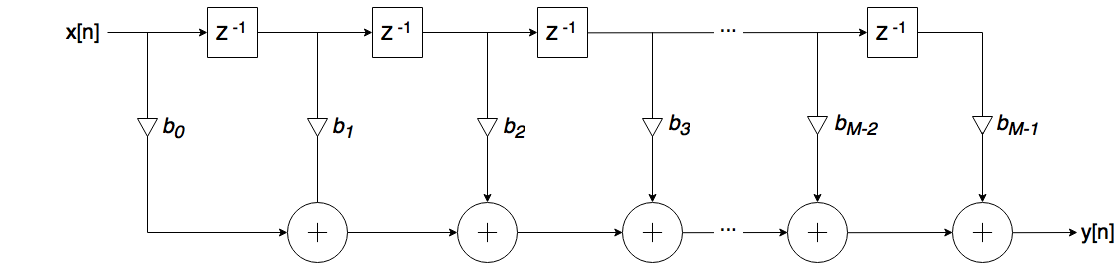
\includegraphics[width=\textwidth]{../figs/FIRFilter.png}
\caption{\label{fig:firfilter}Direct form representation of a N-order FIR-filter.}
\end{figure}


Even though the process of designing a \gls{fir}-filter might not be a trivial task, the implementation of an already designed filter is simple. As seen from \cref{eq:firfilterconv}, the filter can be described by the convolution formula, which implies that the filter can be implemented as convolution of the input function \textit{x(n)} with the impulse response function \textit{h(n)}.
\chapter{Methodology}

\section{\label{sec:legupclasses}LegUp classes}
LegUp has some predefined classes that is important for the understanding of the following description of how the issues in LegUp are resolved. The following subsections will describe these classes in more detail.
\subsection{RTLModule}
The RTLModule class models a hardware RTL module. The class stores information about all ports (inputs and outputs), signals, parameters and sub-modules. Each function declared in the C-code transforms into a RTLModule object. Each function that is called from the function will be added as a sub-module to the RTLModule object, meaning a module instantiation will be added to the module. Important member functions in the RTLModule class is:
\begin{compactdesc}
    \item[getName()] \hfill \\
    Returns a string containing the name of the RTLModule, i.e. "main" for the module generated by the main-function in the C-program.
    \item[find(std::string signal)] \hfill \\
    Takes a string containing a signal name as parameter and returns a pointer to the RTLSignal in the RTLModule with that name.
    \item[addParam()] \hfill \\
    Adds a parameter to the module. The function returns a pointer to the generated RTLSignal object.
    \item[addIn()] \hfill \\
    Adds an input port to the module. The function returns a pointer to the generated RTLSignal object.
    \item[addOut()] \hfill \\
    Adds an output port to the module. The function returns a pointer to the generated RTLSignal object.
    \item[addRegOut()] \hfill \\
    Adds a registered output port to the module. The function returns a pointer to the generated RTLSignal object.
    \item[addReg()] \hfill \\
    Adds a register signal to the module. The function returns a pointer to the generated RTLSignal object.
    \item[addWire()] \hfill \\
    Adds a wire signal to the module. The function returns a pointer to the generated RTLSignal object.
    \item[addModule()] \hfill \\
    Adds a instantiation of another module to the module. The function returns a pointer to the generated RTLModule
    object.
\end{compactdesc}
\subsection{RTLSignal}
The RTLSignal class represents the signals within an RTLModule. Both internal signals, port signals and condition signals are all modelled usign the RTLSignal class. Important member functions of the class is:
\begin{compactdesc}
    \item[getName()] \hfill \\
    Returns a string containing the name of the RTLSignal, i.e. "clk" for the clock signal.
    \item[getType()] \hfill \\
    Returns a string describing the signal type. The type can be reg, wire, input, output and output reg.
    \item[getNumDrivers()] \hfill \\
    Return the number of driving RTLSignals. 
    \item[getDriver(unsigned i)] \hfill \\
    Returns a pointer to the i-th driving RTLSignal.
    \item[getCondition(unsigned i)] \hfill \\
    Returns a pointer to the condition signal of the i-th driving RTLSignal.
    \item[addCondition(RTLSignal *cond, RTLSignal *driver)] \hfill \\
    Adds a conditional driver. If the RTLSignal \textit{cond} is true, the RTLSignal \textit{driver} drives the signal. 
    \item[connect(RTLSignal *s)] \hfill \\
    Connect this signal unconditionally to another RTLSignal.
    \item[getWidth()] \hfill \\
    Returns a pointer to a RTLWidth object, describing the width of the RTLSignal.
    \item[isOp()] \hfill \\
    Returns true if the RTLSignal is an RTLOp object.
\end{compactdesc}
\subsection{RTLOp}
The RTLOp class is a subclass of the RTLSignal class, representing an operation with one, two or three operands. Each operand is a RTLSignal. The operation can be an arithmetic operation like addition, subtraction, multiplication, or division, and it can also be logical operations like AND, OR, and XOR, or even comparison operations like equal, not equal, less than, less than or equal, greater than, and greater than or equal. The whole list can be seen in the class reference \cite{rtlopclassref}. A RTLOp object modelleing an AND operation of two operands, operand1 and operand2, will in Verilog correspond to the operation \verb!operand1 & operand2!. Some important member functions are:
\begin{compactdesc}
    \item[getOperand(int i)] \hfill \\
    Returns a pointer to i-th operand of the RTLOp object.
    \item[getNumOperands()] \hfill \\
    Returns the number of operands of the RTLOp object.
    \item[setOperand(int i, RTLSignal *s)] \hfill \\
    Sets the i-th operand to the RTLSignal \textit{s}.
\end{compactdesc}
\subsection{RTLWidth}
The RTLWidth class represents the bitwidth of a RTLSignal. An RTLWidth is defined by high and low bits, for instance 31,0 for a 32 bit signal. This will transform into \verb![31:0]! in Verilog.
\subsection{RAM}
The RAM class models RAM modules in LegUp. Whenever a variable is loaded or stored, a RAM module is generated to handle the loads and stores. The RAM objects can be divided into two scopes; LOCAL and GLOBAL. A Local RAM object is local to a given function and cannot be accessed from other functions. A global RAM object will be implemented in a global memory controller, and all modules that use the variable can connect to the RAM via the memory controller. Some important member functions are:
\begin{compactdesc}
    \item[getName()] \hfill \\
    Returns a string containing the name of the RTLModule, i.e. "main\_0\_1" for the RAM module generated for the first parameter to the main function declared as volatile (output parameters) in the C-code.
    \item[isROM()] \hfill \\
    Returns true if the RAM is read-only.
    \item[getScope()] \hfill \\
    Returns if the RAM is in the local or global scope.
\end{compactdesc}

\section{LegUp tool-flow example}
To give you a general idea of how LegUp works, this section will give a simple example starting with the C-code and all the way through synthesis and layout. \Cref{lst:ccodelisting} shows a simple C-program with two functions, main and squared. The main function will be the top function and this function takes three input parameters, \textit{done}, \textit{inData} and \textit{\_\_out\_outData}. The main function contains a while loop, which will run as long as the input parameter done is set to zero. Inside the loop the function squared is called with the argument from inData and the return value from squared is assigned to the input argument \textit{\_\_out\_outData}. If you are familiar with C programming, you will see that it is a weird thing to be assigning values to the inputs, but as we will see later in \cref{sec:assValueToOutput}, this is a way to get multiple outputs to the generated module. Notice also the \textit{volatile} keyword in the declaration of the \textit{\_\_out\_outData} parameter, as this is a necessary part of the generating outputs.
\lstset{language=C++,style=Cstyle}
\begin{lstlisting}[caption={Simple C-code example},label=lst:ccodelisting]
int squared (int base) {
  return base * base;
}

int main (int done, int inData, volatile int __out_outData) {
  while(done == 0) {
    __out_outData = squared(inData);
  }
  return 0;
}
\end{lstlisting}

\subsection{HLS with LegUp}
The C-code is compilated into LLVM IR using the clang frontend for the LLVM compilation framework. The initial result before any \gls{lto} is performed is shown in \cref{lst:llvmirprelto}. If you are familiar with assembly code, you might understand some of the operations, like alloca, load, store, mul and icmp. Each define block corresponds to one function from the C-code. The main function, which contains a while-loop, is split into multiple labels. The first section refers to the input parameters and memory allocation and storing of these. Temporary registers, declared on the form \%1, \%2 .. \%N, are inserted where needed. The section from the line "\textit{; <label>:4}" is the checking of the condition of the while loop. Further, \textit{label 7} is operations inside the while loop, and \textit{label 10} is operations after the loop has exited.
\lstset{language=llvm,style=LLVMstyle}
\begin{lstlisting}[caption={LLVM IR before LTO},label=lst:llvmirprelto]
define i32 @squared(i32 %base) #0 {
  %1 = alloca i32, align 4
  store i32 %base, i32* %1, align 4
  %2 = load i32* %1, align 4
  %3 = load i32* %1, align 4
  %4 = mul nsw i32 %2, %3
  ret i32 %4
}

; Function Attrs: noinline nounwind
define i32 @main(i32 %done, i32 %inData, i32 %__out_outData) #0 {
  %1 = alloca i32, align 4
  %2 = alloca i32, align 4
  %3 = alloca i32, align 4
  store i32 %done, i32* %1, align 4
  store i32 %inData, i32* %2, align 4
  store volatile i32 %__out_outData, i32* %3, align 4
  br label %4

; <label>:4                              ; preds = %7, %0
  %5 = load i32* %1, align 4
  %6 = icmp eq i32 %5, 0
  br i1 %6, label %7, label %10

; <label>:7                              ; preds = %4
  %8 = load i32* %2, align 4
  %9 = call i32 @squared(i32 %8) #1
  store volatile i32 %9, i32* %3, align 4
  br label %4

; <label>:10                             ; preds = %4
  ret i32 0
}
\end{lstlisting}
By default, some optimization passes are run on the IR to remove unnecessary operations and reduce the number of registers needed. All available passes are described in \cite{llvmpasses}, but the ones that is run by default is \textit{mem2reg}, \textit{instcombine}, \textit{loops}, \textit{loop-simplify}, \textit{basicaa}, \textit{indvars}, \textit{loop-pipeline}, \textit{internalize}, and \textit{globaldce}. These passes analyses, simplifies and removes operations. The result is listed in \cref{lst:llvmirpostlto}. Notice that the only stores left in the code is the ones connected to the input parameter declared as volatile. The keyword volatile, which definition is \textit{likely to change suddenly and unexpectedly}, tells the compiler to avoid performing optimizations on this object, as it might change in an unexpected way. This is what we want, as assigning values to an input parameter in C does not make sense, and would therefore have been optimized away. 

\begin{lstlisting}[caption={LLVM IR after LTO},label=lst:llvmirpostlto]
define internal i32 @squared(i32 %base) #0 {
  %1 = mul nsw i32 %base, %base
  ret i32 %1
}

; Function Attrs: noinline nounwind
define i32 @main(i32 %done, i32 %inData, i32 %__out_outData) #0 {
  %1 = alloca i32, align 4
  store volatile i32 %__out_outData, i32* %1, align 4
  br label %2

; <label>:2                              ; preds = %4, %0
  %3 = icmp eq i32 %done, 0
  br i1 %3, label %4, label %6

; <label>:4                              ; preds = %2
  %5 = call i32 @squared(i32 %inData) #1
  store volatile i32 %5, i32* %1, align 4
  br label %2

; <label>:6                              ; preds = %2
  ret i32 0
}
\end{lstlisting}

Also notice that the storing and loading of the other input parameters has been swapped by referencing the input parameter register directly. For instance the four lines:

\begin{lstlisting}
%2 = alloca i32, align 4
store i32 %inData, i32* %2, align 4
%8 = load i32* %2, align 4
%9 = call i32 @squared(i32 %8) #1
\end{lstlisting}
has been transformed into the single line:
\begin{lstlisting}
%5 = call i32 @squared(i32 %inData) #1
\end{lstlisting}
The LegUp backend pass for LLVM is run on the IR to generate Verilog-output. LegUp perfomes allocation, scheduling and builds RTL models of the functionality, based on given constraints. These RTL models are printed to a file as Verilog HDL. \cref{lst:verilogmodule1} shows the declaration of the \textit{main}-module, parameters representing states, port and internal signal declarations and instantiation of sub-modules.
\lstset{language=Verilog, style=VerilogStyle}
\begin{lstlisting}[caption={Verilog module, port, signal and parameter declaration, and sub-module instantiation},label=lst:verilogmodule1]
module main
(
	clk,
	clk2x,
	clk1x_follower,
	reset,
	start,
	finish,
	memory_controller_waitrequest,
	return_val,
	arg_done,
	arg_inData,
	arg_outData,
	arg_outData_valid,
	iterationFinish
);

parameter [3:0] LEGUP_0 = 4'd0;
parameter [3:0] LEGUP_F_main_BB__0_1 = 4'd1;
parameter [3:0] LEGUP_F_main_BB__0_2 = 4'd2;
parameter [3:0] LEGUP_F_main_BB__2_3 = 4'd3;
parameter [3:0] LEGUP_F_main_BB__4_4 = 4'd4;
parameter [3:0] LEGUP_F_main_BB__4_6 = 4'd6;
parameter [3:0] LEGUP_F_main_BB__4_7 = 4'd7;
parameter [3:0] LEGUP_F_main_BB__6_8 = 4'd8;
parameter [3:0] LEGUP_function_call_5 = 4'd5;

input  clk;
input  reset;
input  start;
output reg  finish;
input  memory_controller_waitrequest;
output reg [31:0] return_val;
input [31:0] arg_done;
input [31:0] arg_inData;
output reg [31:0] arg_outData;
output reg  arg_outData_valid;
output reg  iterationFinish;
reg [3:0] cur_state;
reg [3:0] next_state;

squared squared (
	.memory_controller_waitrequest (memory_controller_waitrequest),
	.clk (clk),
	.clk2x (clk2x),
	.clk1x_follower (clk1x_follower),
	.reset (reset),
	.start (squared_start),
	.finish (squared_finish),
	.return_val (squared_return_val),
	.arg_base (squared_arg_base)
);
\end{lstlisting}
LegUp generates an FSM that performs calculations and generates output. The generated FSM controller for the above example code is listed in \cref{lst:verilogfsm}, and the state diagram of the FSM is shown in \cref{fig:verilogfsm}.
\begin{lstlisting}[caption={Verilog FSM},label=lst:verilogfsm]
always @(posedge clk) begin
if (reset == 1'b1)
	cur_state <= LEGUP_0;
else if (memory_controller_waitrequest == 1'd1)
	cur_state <= cur_state;
else
	cur_state <= next_state;
end

always @(*)
begin
next_state = cur_state;
case(cur_state)  // synthesis parallel_case  
LEGUP_0:
	if ((start == 1'd1))
		next_state = LEGUP_F_main_BB__0_1;
LEGUP_F_main_BB__0_1:
		next_state = LEGUP_F_main_BB__0_2;
LEGUP_F_main_BB__0_2:
		next_state = LEGUP_F_main_BB__2_3;
LEGUP_F_main_BB__2_3:
	if ((main_2_3 == 1'd1))
		next_state = LEGUP_F_main_BB__4_4;
	else if ((main_2_3 == 1'd0))
		next_state = LEGUP_F_main_BB__6_8;
LEGUP_F_main_BB__4_4:
		next_state = LEGUP_function_call_5;
LEGUP_F_main_BB__4_6:
		next_state = LEGUP_F_main_BB__4_7;
LEGUP_F_main_BB__4_7:
		next_state = LEGUP_F_main_BB__2_3;
LEGUP_F_main_BB__6_8:
		next_state = LEGUP_0;
LEGUP_function_call_5:
	if ((squared_finish_final == 1'd1))
		next_state = LEGUP_F_main_BB__4_6;
default:
	next_state = cur_state;
endcase
end
\end{lstlisting}
\begin{figure}[hbpt]
\centering
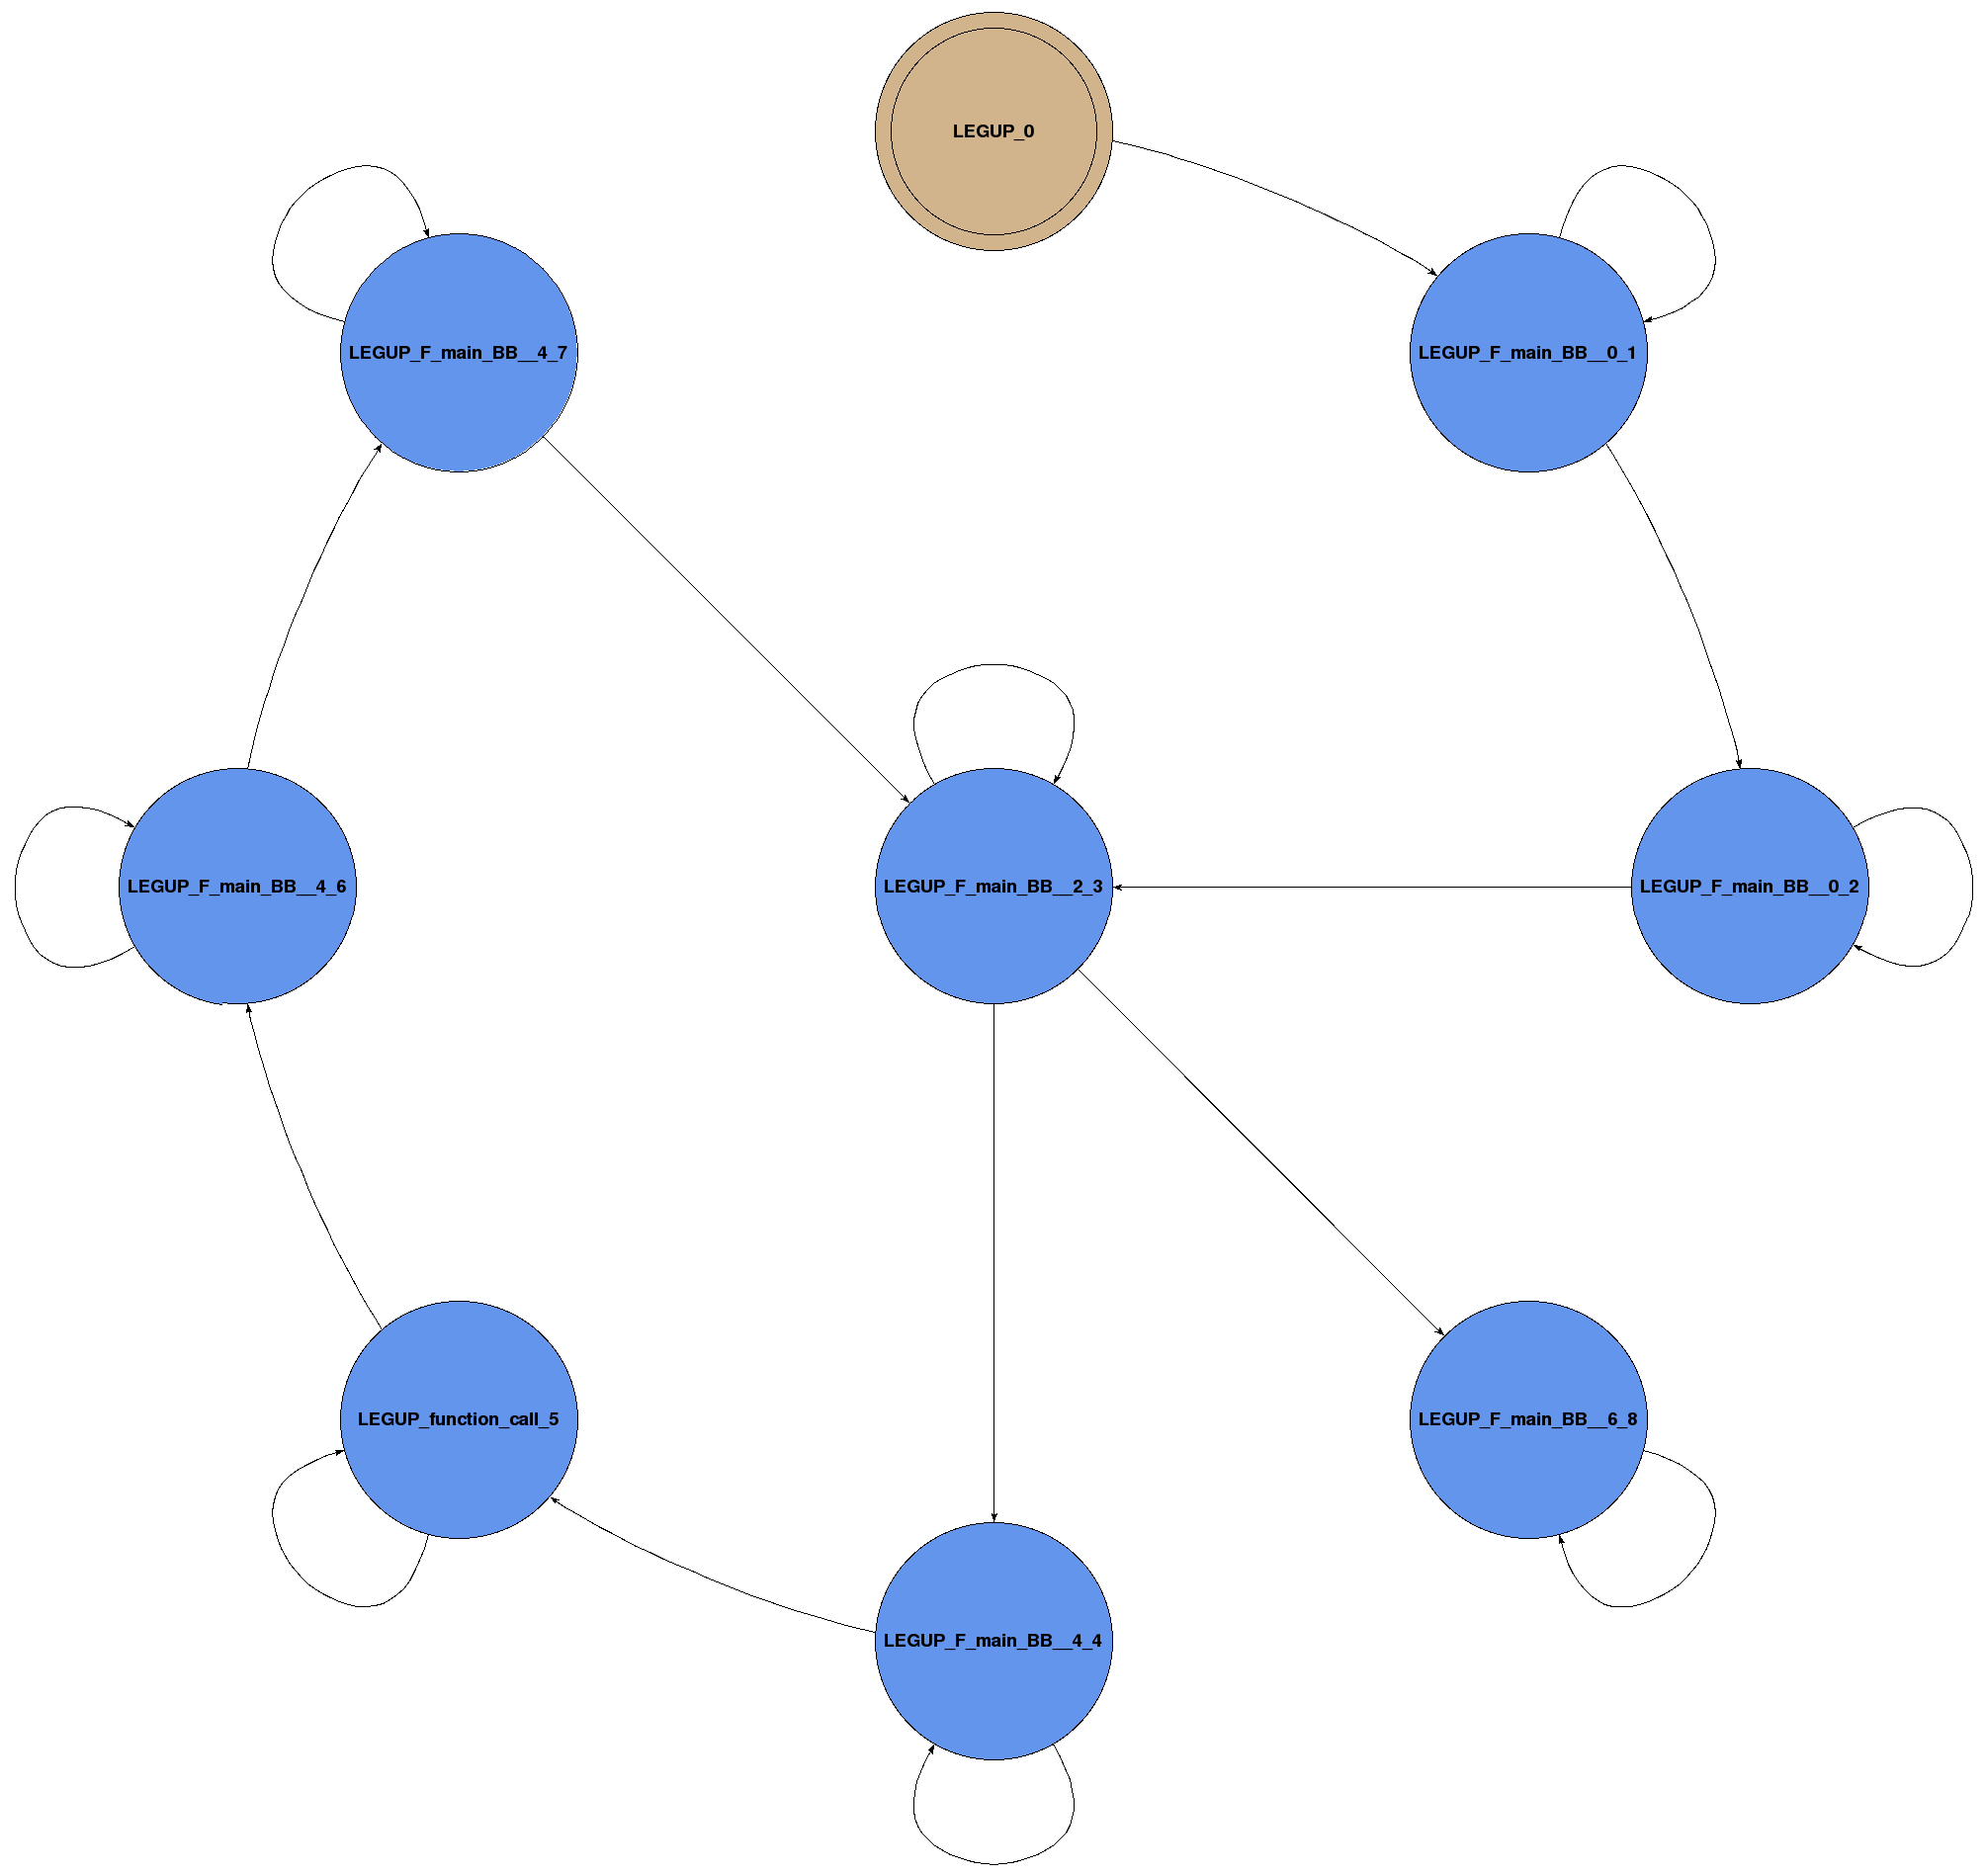
\includegraphics[width=0.9\textwidth]{../figs/VerilogFSM.png}
\caption{\label{fig:verilogfsm}State diagram of generated FSM}
\end{figure}
By looking at the state diagram, some parts from the C-code can be recognized. \textit{LEGUP\_0} is the initial state and the two following states is allocating and storing the volatile input parameter. \textit{LEGUP\_F\_main\_BB\_2\_3} is where the condition checking for the while loop is performed. The states below and left of the condition state is the states inside the while loop, and \textit{LEGUP\_F\_main\_BB\_6\_8} is the exit-state, signalizing the completion of the program.

Some signal assignments are shown in \cref{lst:verilogsignalassignment}. Each assignment is printed with the corresponding LLVM operation commented abowe, to increase readability of the code. The later assignment of output signals are not generated directly from an LLVM operation and does thus not have this operation printed along the assignment.
\begin{lstlisting}[caption={Verilog FSM},label=lst:verilogsignalassignment,float]
always @(*) begin
	/* main: %2*/
	/*   %3 = icmp eq i32 %done, 0*/
		main_2_3 = (arg_done == 32'd0);
end
always @(posedge clk) begin
	/* main: %4*/
	/*   %5 = call i32 @squared(i32 %inData) #1*/
	if ((cur_state == LEGUP_F_main_BB__4_4)) begin
		squared_arg_base <= arg_inData;
	end
end
always @(posedge clk) begin
	if ((cur_state == LEGUP_F_main_BB__4_6)) begin
		arg_outData <= main_4_5_reg;
	end
end
always @(posedge clk) begin
	if ((cur_state == LEGUP_F_main_BB__4_6)) begin
		arg_outData_valid <= 1'd1;
	end
	if (~((cur_state == LEGUP_F_main_BB__4_6))) begin
		arg_outData_valid <= 1'd0;
	end
end
always @(posedge clk) begin
	if ((cur_state == LEGUP_F_main_BB__4_7)) begin
		iterationFinish <= 1'd1;
	end
	if (~((cur_state == LEGUP_F_main_BB__4_7))) begin
		iterationFinish <= 1'd0;
	end
end
\end{lstlisting}

\subsection{Simulation}
\subsubsection{Simulation libraries}

LegUp generates local RAMs for each output-parameter to the main module, as these parameters needs to be declared as volatile. 

In the declaration of the modules ram\_dual\_port and rom\_dual\_port, a conversion function from an Altera library is used to convert .mif files to a format readable by Modelsim. The .mif-file contains initial content of memory. The code snippet that uses this library is shown in \cref{lst:alteralibrary}. If the design does not contain any initial memory values, this conversion method is not needed and could be removed from the design. As this is a feature in LegUp, this has not been altered at this time. This requires the library file to be included in the design filelist for simulation to be successful. The library-file is located in \textasciitilde/legup-4.0/ip/libs/altera/altera\_mf.v of the LegUp VirtualBox image. 
\lstset{language=Verilog, style=VerilogStyle}
\begin{lstlisting}[caption={Altera Library function used for memory management},label=lst:alteralibrary]
ALTERA_MF_MEMORY_INITIALIZATION mem ();
// modelsim can't read .mif files directly. So use Altera function to
// convert them to .ver files
mem.convert_to_ver_file(init_file, width_a, ram_ver_file);
$readmemh(ram_ver_file, ram);
\end{lstlisting}

In the physical implemented design, memory cannot be filled with initial values, and thus this section of code is not included in synthesis, indicated by the commented lines \verb!"synthesis_translate_off"! and \verb!"synthesis_translate_on"!. Also, since the library file is not synthesizable, it cannot be included in the filelist used for synthesis.

\subsubsection{Running simulation}
The generated Verilog code is simulated using QuestaSim. The simulation is executed by running the script \textit{RUN\_ALL} located in the rtl folder. The GUI of QuestaSim can be brought up by passing the argument \verb!-g! to the script, otherwise the simulation will be run in batch mode in the terminal.

To simulate the design, a suitable testbench needs to be provided. Fortunately, LegUp generates a testbench shell, meaning we only need to add the testcases we want to apply to the circuit. Since this is a simple example, we only provide a few testcases to ensure the design works as expected. 
\begin{lstlisting}[caption={Testcases for the example testbench},label=lst:tbcases]
initial begin
    arg_done <= 32'd0;
    arg_inData <= 32'd20;
    
    @(negedge reset);
    start <= 1;
    @(negedge clk);
    start <= 0;
    
    @(posedge iterationFinish);
    arg_inData <= 32'd100;
    
    @(posedge iterationFinish);
    arg_inData <= 32'd498;
    
    @(posedge iterationFinish);
    arg_done <= 32'd1;
end
\end{lstlisting}
\Cref{lst:tbcases} shows the testcases we apply to the circuit. Initial values of the inputs \textit{done} and \textit{inData} is set, and the testbench waits for a falling edge of the reset signal, set by the automatic generated testbench shell, before setting the \textit{start}-flag high for one clock cycle. At the two folloeing rising edges of the \textit{iterationFinished}-flag, a new value is assigned to the input \textit{inData}. At the third rising edge of the \textit{iterationFinished}-flag, the input \textit{done} is set to one, indicating the end of this run. A waveform from the simulation is shown in \cref{fig:simulationwave}. From the waveform we observe that the circuit has the expected behaviour. When the \textit{start}-flag is set, the FSM starts and the sub-module \textit{squared} starts to calculate the output value. When \textit{cur\_state} of the \textit{main}-module equals 7, the calculated value is assigned to the output \textit{outData}, and the \textit{valid}-flag for this output is set. The value on the output is correctly calculated for the given testcases. When \textit{cur\_state} equals 3, the {iterationFinish}-flag is set, as this is the state where the condition for the while loop is evaluated, i.e. one iteration of the loop is complete. Notice that the \textit{iteartionFinish}-flag is not set in the first occurrence of \textit{cur\_state} = 3, as this is the first encounter of the loop and not a finished iteration. When the input \textit{done} is set to 1 after the third \textit{iterationFinish}-flag, we observe that the loop terminates and the \textit{finish}-flag is set, indicating the end of the run.
\begin{figure}[hbpt]
\centering
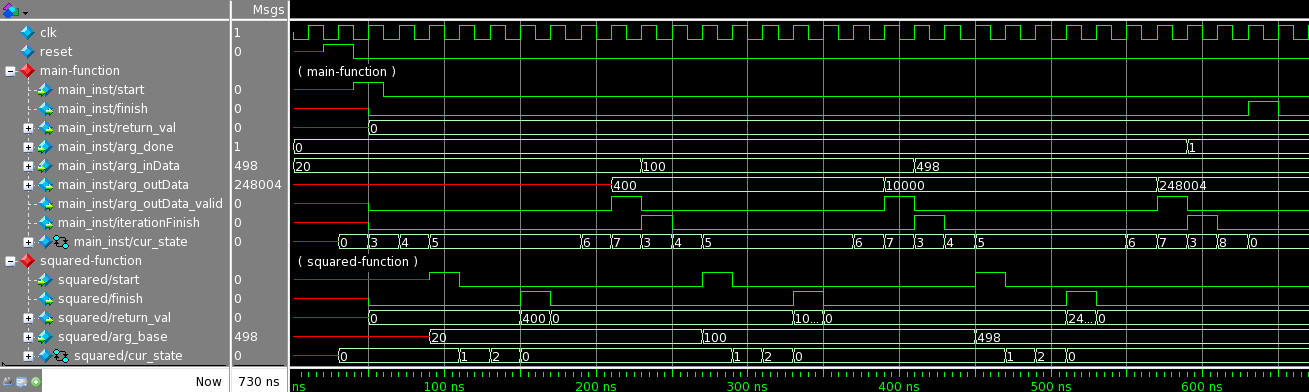
\includegraphics[width=0.99\textwidth]{../figs/SimulationWaveEX.png}
\caption{\label{fig:simulationwave}Simulation waveform of example design}
\end{figure}
\subsection{Synthesis}
The design is synthesized using a 180nm library. The area and frequency reports from the synthesis is presented in \cref{tab:synthreportex}.
\begin{table}[]
    \centering
    \begin{tabular}{lcr}
        \textbf{Parameter} && \textbf{Value} \\
        \toprule
        Number of ports && 137 \\
        Number of nets && 906 \\
        Number of cells && 505 \\
        Number of combinational cells && 371 \\
        Number of sequential cells && 133 \\
        Number of macros/black boxes && 0 \\
        Number of buf/inv && 135 \\
        Number of references && 31 \\
        \midrule
        Combinational area && 26740.929852 \\
        Buf/Inv area && 3466.108790 \\
        Noncombinational area && 20824.373009 \\
        Macro/Black Box area && 0.000000 \\
        Net Interconnect area && 39816.683686 \\
        \midrule
        Total cell area && 47565.302861 \\
        Total area && 87381.986547 \\
        \midrule
        Critical Path Length && 77.71 ns \\
        Maximum Frequency && 12.86 MHz\\
        \bottomrule
    \end{tabular}
    \caption{Caption}
    \label{tab:synthreportex}
\end{table}
To put the area of the synthesized design in perspective, the library defines a two-port NAND gate to be 9.9792 area units. The number of NAND2-equivalent gates for the design is then 8757 gates. This is a large amount for such a simple design, but the area overhead percentage of the design will shrink with larger designs. The reported \subsection{Layout}

\subsection{Power estimation}

\subsection{Constraint files}
LegUp uses constraint files to set constraints and settings for the \gls{hls}. The default values for necessary constraints is set in the default constraint-file located in \textasciitilde/legup4-0/example/legup.tcl. The default constraints can be overridden by adding a local constraint file. The filename of the local constraint file need to be specified in the Makefile for the constraints to take effect. This is done by adding the line \verb!LOCAL_CONFIG = -legup-config=config.tcl! to the Makefile, where config.tcl is the filename of the local constraint-file. 
\subsection{Makefile}
The minimal local Makefile of LegUp contains the following three lines:
\begin{verbatim}
  NAME=name
  LEVEL = ..
  include $(LEVEL)/Makefile.common
\end{verbatim}

The Variable \textit{NAME} is the name of the design. This variable will be used to name the output-files of the design. The Variable \textit{LEVEL} indicated the number of directory levels it is up to where the common Makefile is located. 1 level up is marked as .., 2 levels up is marked as ../.. and so on, just like in a standard Linux shell. Other parameters, like \textit{NO\_OPT} (disable optimization in the compilator) and \textit{NO\_INLINE} (avoid inlining functions in the program), can also be added to the Makefile for passing flags and settings to the compilation. In some cases, especially with simple test-programs, these two flags are necessary to prevent the compiler from optimize away the whole program.
%\chapter{Results and discussions}
\label{chp:resdisc}
This chapter will present and discuss achieved results and problems encountered throughout the work with the thesis. Due to the encountered problems, no synthesis or comparison of results from the reference designs have been done, and will therefore not be presented. This should however be easy to perform when the described problems are solved. Some potential solutions to the problems will be presented in \cref{sec:futurework}.
\section{HLS output from LegUp}
\label{sec:legupoutput}
As a quick introduction to how the output from LegUp looks, we will have a look at a simple example. Since the code output is very large, it will be of more use to look at a figure describing the different parts of the code and how it is connected. Beware that this section describes output from LegUp after a fresh installation, without any alterations or changes to settings. In general, the modules declared in the output Verilog file are these:
\begin{compactdesc}
    \item[top]Top-level module. Instantiates \textit{main}- and \textit{memory\_controller}-modules.
    \item[main]\textit{Main}-function from C project. Contains the \gls{fsm} that handles all functionality from the input C program.
    \item[ram\_dual\_port] Dual port RAM module used inside memory controller for global memories.
    \item[rom\_dual\_port] Dual port ROM module used inside memory controller for global memories.
    \item[memory\_controller]Contain global memories and logic for reading and writing to memory. Instantiates necessary \textit{ram\_dual\_port} and \textit{rom\_dual\_port} modules.
    \item[circuit\_start\_control]FPGA specific module. 
    \item[hex\_digits]FPGA specific module. Controls hex LEDs for visualization of results.
    \item[\%board\%]FPGA specific top module. Instantiates top-module and 8 hex{\textunderscore}digits modules and connects return\_value from top to hex modules for visualizing the results.
    \item[main\_tb]Basic testbench that can be used for simulation. Instantiates top-module. Testbench code generates \textit{clk} signal and applies \textit{reset} and \textit{start} signals to the module before waiting for finish flag. There are no additional input stimuli, so this needs to be added manually by the user.
\end{compactdesc}

\noindent
Listing \ref{lst:exampleCProgram} shows a simple C implementation of a square-root approximation method. The reason that the arguments to the \textit{main}-function are given in this way, is described in \cref{subsec:inoutprobs}. \gls{hls} is performed by running \verb!make! in a terminal window. The output Verilog file contains over 3000 lines of code and can therefore not be presented her, it would anyway not give much information. The \gls{ir} from LLVM is shown in \cref{lst:llvmir} for reference.
\lstset{language=C,style=Cstyle}
\begin{lstlisting}[caption={C example: square-root approximation},label=lst:exampleCProgram]
#define abs(a) ( ((a) < 0) ? -(a) : (a) )
#define max( a, b ) ( ((a) > (b)) ? (a) : (b) )
#define min( a, b ) ( ((a) < (b)) ? (a) : (b) )

// square-root approximation:
int main(int inDataA, char *inDataB[]) {
    int x = max(abs(inDataA), abs(*inDataB[0]));
    int y = min(abs(inDataA), abs(*inDataB[0]));
    return max(x, x-(x>>3)+(y>>1));
}
\end{lstlisting}
\noindent
A project in Quartus can be created by running \verb!make p! and a full compilation can be executed by running \verb!make f!. Synthesis of the example in \cref{lst:exampleCProgram} generates a large netlist with many gates and signals, which is hard to read. A simplified diagram only showing the interesting signals and connections from the synthesis output, have therefore been created and can be seen in \cref{fig:legupouttop}.
\begin{figure}[hbpt]
\centering
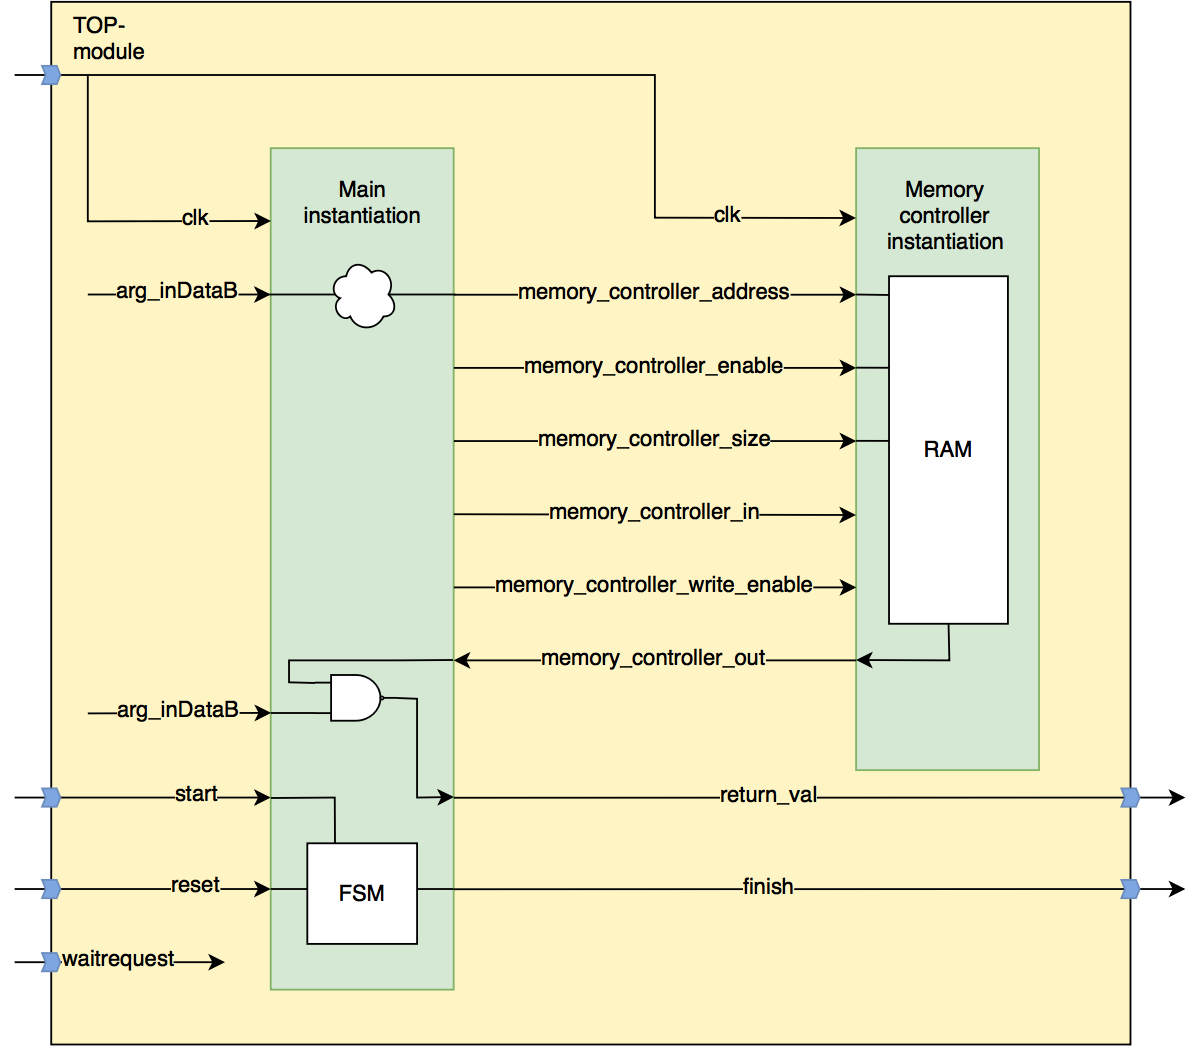
\includegraphics[width=\textwidth]{../figs/LegUpOutputTop.png}
\caption{\label{fig:legupouttop}Top-level module of HLS-generated Verilog from LegUp synthesized in Quartus.}
\end{figure}
Notice that the inputs to the instantiated \textit{main} module, \textit{inDataA} and \textit{inDataB} does not propagate to the top module instantiation. Also, if we look inside the \textit{main} module, \textit{inDataB} is only mapped to the signal \textit{memory\_controller\_address}. The sky-image indicates that something happens inside the module, it is not a direct connection through, but essentially this is what happens. This is because \textit{inDataB} is declared as a pointer in the C code, meaning that the input only provides the address to a location in memory where the data can be fetched. This issue is discussed further in \cref{sec:encprob}.

The signal connections between the main module and the memory controller is described in \cref{tab:hlsoutputsignals}. As the memory controller is dual-ported, two connections for each signal is used, distinguished by the suffix \textit{\_a} and \textit{\_b} for port A and port B respectively. Each memory signal starts with the prefix \textit{memory\_controller\_}.

\begin{table}[hbpt]
    \centering
    \caption{\label{tab:hlsoutputsignals}Description of signals connecting main and memory controller module in HLS-generated Verilog.}
    \begin{tabular}{ll}
      \textbf{Memory signal} & \textbf{Description}\\
      \toprule
      address & 32-bit address of memory \\
      \hline
      enable & Enable signal for memory controller \\
      \hline
      write\_enable & Perform write-operation if high, read operation if low\\
      \hline
      size & Byte-enable signal (write or read single bytes)\\
      \hline
      in & Data input to memory (memory write operations)\\
      \hline
      out & Data output from memory (memory read oeprations)\\
      \bottomrule
    \end{tabular}
\end{table}

\section{\label{sec:encprob}Encountered problems}
Throughout the work with LegUp, multiple problems that limits its usefulness towards \gls{asic}-applications has been encountered. The following section will describe some of the problems and their implication for the continuation of the project.
\subsection{\label{subsec:memctrl}Memory controller}
In order to communicate between different modules instantiated in the top-level module of the Verilog output from LegUp, a memory controller is declared and instantiated. All variables detected as global by LegUp, i.e. variables used by multiple modules or declared as a pointer and the points-to analysis fails to determine the exact array for the pointer at compile-time, is stored in a \gls{ram} module inside this memory controller. This approach is well intended for the hybrid flow supported by LegUp, where a soft-processor works in cooperation with one or more functions implemented as hardware accelerators in an \gls{fpga}. In this flow, the data needs to be transferred between the software and hardware portion of the system. For an \gls{asic}, pure-\gls{hw} implementation however, this approach creates a lot of extra overhead and basically does not provide any additional functionality to the circuitry. In the pure-\gls{hw} flow in LegUp, all the functionality described under the \textit{main}-function in the input C code will be translated into a single \gls{fsm}. The \textit{main}-function is further the only module instantiated in the top-module of the produced Verilog, besides the memory controller. The use of the memory controller is in itself not an issue as LegUp handles all memory access automatically, but this will come at the expense of both decreased speed and increased area usage. It will also cause some problems related to input and output, as described in subsection \ref{subsec:inoutprobs}.

\subsection{\label{subsec:inoutprobs}Inputs and outputs}
The task of a hardware module can vary almost infinitely, however most modules follow the same principle; the module gets some data input together with a set of control signals, processes the data and outputs a result or response. This makes input and outputs, and the ability to configure them properly, extremely important in most module design. In the documentation of LegUp \cite{leguparch}, the developers claim that each function declared in C is translated into a corresponding module in Verilog. However, \gls{hls}-output shows that in the pure-\gls{hw} flow, the only generated module is the one containing the \textit{main}-function, as describe in subsection \ref{subsec:memctrl}. As LegUp uses a standard C compiler frontend for LLVM to compile the C code into LLVM-\gls{ir}, we need to follow the \gls{ansi}-C specification \cite{isoc} when writing our C code. In a standard programming case, the \textit{main}-function has a special purpose, specifically, the run-time environment calls this function to start execution of the program. The return value of the \textit{main}-function is defined to be an integer (int), whose purpose is to return program execution status to the invoker process. The \textit{main}-function is also defined to handle arguments input from command-line, through the input arguments \textit{int argc} and \textit{char *argv[]}, where \textit{argc} is the number of command-line arguments, and \textit{*argv} is an array of pointers to the given arguments. The implications of this is that if we want inputs and outputs to or from the module we design in out C code, we are limited to the arguments allowed through the defined \textit{main}-function in the \gls{ansi}-C specifications. This problem increase when we realize that almost any inputs or outputs have to be pointers, meaning it has to go through the above described memory controller. This causes a lot of overhead, as most input- and output-data has to be written to and read from memory, creating the need for a dedicated custom module for handling I/O. Also, returning a value in C by calling the \textit{return}-function, will terminate the program. This means that a value might not be output until the program is done. One more issue related to input signals, is that the given arguments to the \textit{main}-function in C are not propagated from the generated main module to the top-level module to make them inputs to the circuit. This means that the designer has to manually alter the generated Verilog to make the the arguments input signals, making it more difficult to create the desired automated framework.

\subsection{Bus widths}
When designing digital hardware circuits, you often want (and in some cases need) to use bit-vectors of a given size. \gls{ansi}-C does not have built-in support for data-types of other sizes than 8, 16, 32 and 64 bits, this cause problems when doing \gls{hls}. LegUp has a class, \textit{MinimizeBitwidth.cpp}, which calculate the minimum needed bits in a signal and limits the width to this size, but this does only work for internal signals, where all values assigned to the variable is known at compile-time. If the signal shall be an input or output, the maximum value of the signal is not known, and it can therefore not be limited. Having too wide signals will increase the occupied area as all components must support the extra bits. A simple example is shown in figure \ref{fig:andgate34}, where we can easily see that the addition of one extra bit to the input signal adds one extra 2-input AND gate to the circuit. Technically this is a limitation inherited from the lack of logical data-types in C, but this problem needs to be addressed if LegUp shall be used in an architectural exploration framework.
\begin{figure}[hbpt]
\centering
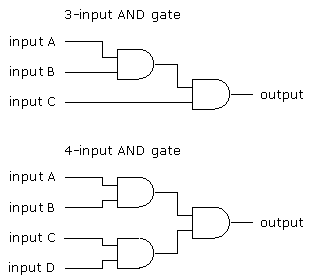
\includegraphics[width=0.6\textwidth]{../figs/AndGate34Bit.png}
\caption{\label{fig:andgate34}3-bit input versus 4-bit input AND-gate.}
\end{figure}

\subsection{\label{subsec:parameterprobs}Parameters}
When designing a module, it has become more and more common to design for reuse and parametrization of sizes. The lack of support for transferring parameters from the C code into the generated Verilog makes it harder to instantiate modules based on widths or depths of different parameters. This is not a problem for the architectural exploration usage of the tool, as the final implementation will be done in a \gls{hdl}. It is possible to generate multiple modules by changing the sizes in the C code, but it would be a nice feature to support parameters if LegUp should be used to generate actual hardware. The problem with parameters in this case, is that the generated \gls{fsm} only accounts for the specified width of signals etc., when generating the necessary operation-resources in the circuit.

\section{Tool-flow and script}
One of the objectives of this thesis was to create a script, making it possible to run the entire process of \gls{hls}, synthesis, and power estimation automatically. Due to the above mentioned problems, this objective has not been fulfilled. Since the \gls{hls}-tool, LegUp, is located on a VirtualBox image, while the synthesis and power estimation tools are located on Nordic Semiconductor's servers, it is not possible to make a single tool-flow that can be run on one computer. A possible solution to create a single tool-flow can be to connect to the LegUp image and run commands remotely from Nordic's servers using the \gls{ssh}-protocol. File transfers to and from the image can be performed using the \gls{scp}, which is included in most \gls{ssh} implementations.
%\chapter{Conclusion}
\label{chp:conclusion} 
This report has presented the \gls{hls}-tool, LegUp, and shown how it potentially can be used in a framework for architectural exploration of digital hardware toward \gls{asic} applications. A specification of a framework that can be used to automate the process of architectural exploration have been presented. Unfortunately, multiple problems were encountered along the way. Identifying and attempting to resolve these problems required a lot of time, which took the focus away from the main objectives. The outcome of this, is that no results from comparison between hand-written Verilog and \gls{hls} generated Verilog are presented. The implementations of the designs are still presented, making it an easy task to do the comparison once the encountered problems are sorted out.

In its current state, LegUp cannot be used as a tool for architectural exploration of digital hardware in the context of \gls{asic} applications. For this, it has too many elementary deficiencies which are required when designing hardware for an \gls{asic} implementation. If LegUp can be used for our initial intentions, cannot be concluded until the presented issues have been resolved and a larger "proof-of-concept"-study has been conducted. The major advantage LegUp has is that it is open-source and thus, it has the potential to become whatever you want it to be - given that you have time to do it yourself. However, it is important to remember that transforming a tool into something it is not intended for, might be more time-consuming than creating what you need from scratch.

The following section will present future work for an eventual continuation of the project. Some fundamental issues that needs attention are described firstly. The issues are followed by two proposed approaches to eliminate the problems, and solutions for some of the issues for each approach. Finally, a list of further extensions are included. These extensions are not vital for the use of LegUp in an architectural exploration framework, but they add functionality that any designer would cherish.
\section{Future work}
\label{sec:futurework} 


\subsection{Required actions}
\label{subsec:reqact}
If this project should be extended into a master thesis or project at a later stage, the following issues needs to be handled:
\begin{enumerate}
    \item \label{item:futworkprob}The Clang frontend in LLVM, used by LegUP for compilation of the C-source code, needs to be altered so that the list of input variables and return values in the \textit{main}-function of the C program can be of other formats than the standard \textit{int main(int argc, char *argv[])}.
    \item Pointers in the C program needs to be transformed into signals instead of a memory location inside the memory controller. As there is only one module in the output Verilog, no point-to analysis is needed to decide what module the pointed variable will be used in. This will eliminate the need for the memory controller and global \gls{ram}s.
    \item The memory controller module, as well as all other unused, \gls{fpga} specific modules, need to be removed from the Verilog generation. Theses modules are not needed when there is no hybrid-flow, and pointers no longer are stored in global memory. The most important task is to ensure that the modules are not instantiated in the top module, but having multiple unused modules declared in the Verilog code clogs up the file with unnecessary lines, making it harder to detect actually important parts.
    \item A way to specify the bit-width of a signal must be implemented. Since no other sizes than 8, 16, 32, and 64 bits are supported by \gls{ansi}-C, new data-types have to be defined in C, or a way to set constraints on input/output signals must be added to LegUp.
\end{enumerate}

\subsubsection{Possible solutions}

There are two possible approaches in order to fix these problems:
\begin{itemize}
\item Post-processing of the Verilog generated by LegUp, in order to remove unwanted code and adapt the code into a format suitable for synthesis towards an \gls{asic} implementation.
\item Pre-processing, i.e. altering the LegUp and LLVM libraries that are used for compilation of the source code and Verilog generation, so that the output Verilog are synthesizable to \gls{asic} applications.
\end{itemize}

The post-processing solution is clearly the simplest alternative, as it only requires a parser that can loop through the code and remove or reformat code output. This alternative is however very uncertain with respect to the quality of results. The question is whether or not the Verilog contains enough information to transform it into the desirable format and still keep the correct functionality. The performance might also be a concern, as we will see below.

As an example, we can use the code described in \cref{lst:exampleCProgram} as a base. In the output Verilog code the input variables, inDataA and inDataB, are declared differently, as inDataA is declared as an int while inDataB is declared as a char-pointer in the C program. The output gives:
\lstset{language=Verilog, style=Verilogstyle}
\begin{lstlisting}
input [31:0] arg_inDataA;
input [`MEMORY_CONTROLLER_ADDR_SIZE-1:0] arg_inDataB;
\end{lstlisting}
Later in the Verilog code, the signal inDataA is used as a normal variable, but each time inDataB is used, the value of inDataB is assigned to the output \textit{memory\_controller\_add-ress\_a}, and in the next cycle, the data is sent from the memory controller to the input \textit{memory\_controller\_out\_a} of the \textit{main} module. In this case, the post-processor needs to change the declaration of \textit{inDataB} to be a signal in the circuit, rather than a connection to the memory controller:
\begin{lstlisting}
input [31:0] arg_inDataA;
input [31:0] arg_inDataB;
\end{lstlisting}
The parser also needs to modify the part of the code where the value of inDataB, gathered from the memory controller, is used in operations inside the main module. For instance, the following code snippet in the generated Verilog, assigning the value of inDataB from the memory controller (the commented line refers to the LLVM-\gls{ir}):
\begin{lstlisting}
/*   %36 = load i8** %inDataB, align 4*/
main_35_36 = memory_controller_out_a[`MEMORY_CONTROLLER_ADDR_SIZE-1:0];
\end{lstlisting}
should be changed to:
\begin{lstlisting}
/*   %36 = load i8** %inDataB, align 4*/
main_35_36 = arg_inDataB[31:0];
\end{lstlisting}
This simple example shows what needs to be changed in order to get the correct functionality. This is however not the only part that should be changed. Each access to a global memory takes two clock cycles \cite{leguparch}, meaning that the generated \gls{fsm} takes account for this delay. The delay will have to be eliminated in order to get the best performance out of the circuit. If it is not removed, and the user is not aware of the delay, input data might be lost.

The outcome of this is that the parser needs to account for a large amount of potential alterations in the output Verilog, making it a complex task to get everything correct.

Unless a way of setting constraints on input/output signals are added to LegUp, it is not likely that the parser is able to do anything with the potentially over-sized bit-widths of signals. If the widths of signals are set in a constraint file, the parser can easily change the widths of the signals in the output Verilog-file.

The alternative of altering the LegUp and LLVM libraries, offers much greater opportunities for you to get a functional and correct Verilog output. The downside of this alternative is that the LegUp libraries are quite large, and searching, understanding and altering large parts of the code can be time-consuming. 

A possible solution to the problem mentioned in \cref{item:futworkprob} in \cref{subsec:reqact} has been found. By adding the flag \textit{-ffreestanding} to the variable CLANG\_FLAG in the file Makefile.config of LegUp, the clang compiler frontend of LLVM will consider the C code to contain a freestanding - not a hosted - environment, and therefore not caring about what types of inputs and return values the \textit{main}-function has. This will allow multiple input arguments of any type. You will still be limited to one return variable, as C does not support multiple return values. The return value can be a struct, but due to the limited support for structs, it is not likely that LegUp splits the variables in the struct into multiple output signals in the generated Verilog. The alternative is to use pointers as input arguments, making it possible to get output variables as \textit{pass-by-reference} values. This will probably require major alterations to the LegUp libraries.   

Removing the memory controller from the LegUp libraries might be a complex operation, but it can actually be simpler than in the post-processing option. The libraries that detect if a signal or pointer, points to a single, multiple or unknown function(s), needs to be changed so all point to the \textit{main}-function. This point-to analysis is performed in the file \textit{Allocation.cpp}, and variables are added to local or global \gls{ram}s by the functions below, where \textit{ram} is a pointer to a \gls{ram} object and \textit{F} is a pointer to a function object:
\lstset{language=C,style=Cstyle}
\begin{lstlisting}
/* Adding Local RAM: */
addLocalRam(F, ram);
/* Making RAM global: */
addGlobalRam(ram);
\end{lstlisting}

The memory controller and \gls{fpga} specific modules that are no longer needed can easily be removed from the generated Verilog by removing the printing of the declarations and instantiations in the file \textit{VerilogWriter.cpp}.

\subsection{Optional tasks}

One of the questions raised in the motivation section in the introduction chapter was whether the incorporation of Nordic Semiconductor's \gls{ddvc} into the Verilog generating libraries of LegUp would reduce the generated overhead. As this was not an objective of this project, this extension should be performed in an continuation of the project.

When setting the constraint \textit{INFERRED\_RAMS}, as described in \cref{subsec:hlsreqconst}, the support for structs are lost. This constraint is needed since altsyncram modules are not supported by non-Altera devices. The support for structs are a strength in \gls{hll}-languages that can be useful in many cases when describing the circuit functionality in the C-code before \gls{hls}. According to \cite{legupconst} this lack of struct-support is due to that there is no byte-enable support in the inferred RAMs. Byte-enable means being able to write a single byte (8 bits) to the \gls{ram} instead of the full 32-bit word. To retrieve the support for structs, a generic \gls{ram} module with byte-enable support needs to be implemented in Verilog and incorporated into the LegUp libraries as an alternative to the inferred generic \gls{ram}s and the altsyncram. A template from the Quartus II software, implementing a true dual-port \gls{ram} with different read/write addresses, single read/write clock, and with a control for writing single bytes into the memory word; byte enable, is listed in \cref{sec:ramtempcode}.

The supported output from LegUp is currently limited to Verilog \gls{hdl}. Verilog still gets the job done, but many companies, including Nordic Semiconductor, have moved to SystemVerilog for their preferred design \gls{hdl}. SystemVerilog is the natural successor of Verilog, providing support for user-defined types, adding strong-typing capabilities (for user-defined types), extending capabilities of reuse functionality, greater testbench development, assertion-based verification, and interface abstraction and packaging \cite{bailey2003comparison}. In many cases, SystemVerilog use the same syntax as Verilog, and it should therefore be a simple and natural development to add support for generating SystemVerilog \gls{hdl} output in LegUp.

Another interesting topic is to look into the possibility of extending the basic testbench generated by LegUp, to include automatic generation of test-cases. As the functionality of the module is described in a \gls{hll}, it should be possible to utilize this model to generate a self-checking testbench. This will eliminate the need for writing a custom testbench for each design. A large amount of test-cases are needed for simulation, to provide a realistic \gls{vcd}-file to the power estimation tool. This task might be complex, but if implemented successfully it can decrease the total design-time of a module even further.
%% include here the other chapters

\renewcommand*{\bibname}{References}
%\bibliographystyle{plain}
\bibliographystyle{plainnat}
\bibliography{main}

%% Uncomment the following if you have any appendix
 \appendix
 \addtocontents{toc}{%
  \protect\vspace{1em}% 
  \protect\noindent \bfseries \appendixtocname\protect\par
  \protect\vspace{-.5em}%
 }
 \renewcommand{\chaptername}{\appendixname}
%% include below possible appendices (chapters)

%\chapter{Appendix}
\section{\label{sec:sourcecode}Reference design source codes}

\subsection{FIR-filter - Verilog}
\lstset{language=Verilog, style=Verilogstyle}
\begin{lstlisting}[caption={FIR-filter implemented in Verilog},label=lst:firfilterverilog]
module VerilogFIR (
		ck,
		arst,
		dataIn,
		dataOut
	);
	input ck, arst;
	input signed [WIDTH-1:0] dataIn;
	output reg signed [2*WIDTH-1+$clog2(DEPTH):0] dataOut;
	
	parameter	WIDTH = 32;
	parameter	DEPTH = 4;
	parameter logic signed [WIDTH-1:0] COEFF [DEPTH-1:0] = {1,2,3,4};
	
	reg signed [WIDTH-1:0] sr [DEPTH-2:0];
	reg signed [2*WIDTH-1:0] products [DEPTH-1:0];
	reg signed [2*WIDTH-1+$clog2(DEPTH):0] sum;
	
	always @(posedge ck or arst) begin
		if(arst == 1'b1) begin
			sum = 0;
		end 
		else begin
			sr[0] <= dataIn;
			sr[DEPTH-2:1] <= sr[DEPTH-3:0];
		end
	end
	
	always @* begin
		for (int i = 1; i < DEPTH; i++)
			products[i] = sr[i-1] * COEFF[i];
	end
	
	always @* begin
		sum = products[0];
		for (int i = 1; i < DEPTH; i++)
			sum = sum + products[i];
	end
	
	assign dataOut = sum;
endmodule
\end{lstlisting}
\clearpage
\subsection{FIR-filter - C}
\lstset{language=C,style=Cstyle}
\begin{lstlisting}[caption={FIR-filter implemented in C},label=lst:firfilterc]
#define WIDTH 32  //implicit from the use of ints as input,
#define DEPTH 4

int main(int inData, char **test){
    int sr[DEPTH-1];
	int products[DEPTH];
    int coeff[DEPTH] = {1,2,3,4};

    int sum;
	int i, j;
	products[0] = dataIn * coeff[0];
	sum = products[0];
    for (i = 1; i <= DEPTH; i++){
		for(j=DEPTH-2; j >= 1; j-=1 ){
			sr[j] = sr[j-1];
		}
		sr[0] = inData;
		for (j = 1; j < DEPTH; j++){
			products[i] += sr[j-1] * coeff[j];
		}
        sum += products[i];
    }
    return sum;
}
\end{lstlisting}
\clearpage
\subsection{SAP-1 architecture - Verilog}
\lstset{language=Verilog,style=Verilogstyle}
\begin{lstlisting}[caption={SAP-1 architecture implemented in C},label=lst:sap1archverilog]
module Sap1ProgramCounter (ck, arst, cp, ep, wbus);
	parameter 					BUS_WIDTH 	= 8;
	input 						ck, arst, cp, ep;
	output	[BUS_WIDTH/2-1:0]	wbus;
	reg		[BUS_WIDTH/2-1:0]	pc;
	always @ (posedge ck)
	begin
		if(arst)		pc = 4'b0000;
		else if (cp)	pc = pc + 1;
	end
	assign wbus = ep ? pc : 4'bzzzz;
endmodule

module Sap1MemoryAddressRegister(ck, lm_n, ramAddress, wbus);
	parameter 					BUS_WIDTH 	= 8;
	parameter 					ADDR_WIDTH 	= 4;
	input 						ck, lm_n;
	input	[BUS_WIDTH/2-1:0]	wbus;
	output	[ADDR_WIDTH-1:0]	ramAddress;
	reg		[ADDR_WIDTH-1:0]	ramAddress;
	always @ (posedge ck)
	begin 
		if(!lm_n)	ramAddress = wbus;
	end
endmodule 

module Sap1Ram(ck, ce_n, addr, wbus);

	parameter 					BUS_WIDTH	= 8;
	parameter 					ADDR_WIDTH	= 4;
	input 						ck, ce_n;
	input	[ADDR_WIDTH-1:0]	addr;
	inout	[BUS_WIDTH-1:0] 	wbus;
	reg		[BUS_WIDTH-1:0] 	dataout;
	reg		[BUS_WIDTH-1:0] 	rammem[0:2**ADDR_WIDTH];
	always @ (ce_n)      //asynchronous RAM
	begin 
		dataout <= !ce_n ? rammem[addr] : 8'bz;
	end
	assign wbus = dataout;

endmodule

module Sap1InstructionRegister(ck, arst, li_n, ei_n, opcode, wbus);
	parameter 					BUS_WIDTH = 8;
	input 						ck, li_n, ei_n, arst;
	inout	[BUS_WIDTH-1:0] 	wbus;
	output	[BUS_WIDTH/2-1:0]	opcode;
	reg		[BUS_WIDTH-1:0]		wbusOut;
	reg		[BUS_WIDTH-1:0]		instructionRegister;
	
	always @(posedge ck)
	begin
		if (arst)
		begin 
			instructionRegister <= 8'b0;
		end
		else if(!li_n) 
		begin
			instructionRegister <= wbus;
		end
	end
	assign wbus = !ei_n?{4'b0,instructionRegister[BUS_WIDTH/2-1:0]}:8'bz;
	assign opcode = instructionRegister[BUS_WIDTH-1:BUS_WIDTH/2-1];
endmodule

module Sap1AccumulatorA (ck, la_n, ea, registerA, wbus);
	parameter 				BUS_WIDTH = 8;
	input 					ck, la_n, ea;
	inout	[BUS_WIDTH-1:0]	wbus;
	output 					registerA;
	reg		[BUS_WIDTH-1:0]	registerA;
	always @(posedge ck)
	begin 
		if(!la_n) 
		begin
			registerA <= wbus;
		end
	end
	assign wbus = ea?registerA:8'bz;
endmodule

module Sap1AddSub(su, eu, registerA, registerB, wbus);
	parameter 				BUS_WIDTH = 8;
	input 					su, eu;
	input	[BUS_WIDTH-1:0] registerA, registerB;
	output	[BUS_WIDTH-1:0] wbus;
	assign wbus = eu?(su?registerA-registerB:registerA+registerB):8'bz;
endmodule

module Sap1BRegister(ck, lb_n, registerB, wbus);
	parameter 				BUS_WIDTH = 8;
	input 					ck, lb_n;
	input	[BUS_WIDTH-1:0] wbus;
	output	[BUS_WIDTH-1:0] registerB;
	reg		[BUS_WIDTH-1:0] registerB;
	always @ (posedge ck)
	begin 
		if(!lb_n) registerB = wbus;
	end
endmodule

module Sap1OutputRegister(ck, lo_n, out, wbus);
	parameter 				BUS_WIDTH = 8;
	input 					ck, lo_n;
	input	[BUS_WIDTH-1:0] wbus;
	output	[BUS_WIDTH-1:0] out;
	reg		[BUS_WIDTH-1:0] out;
	always @ (posedge ck)
	begin 
		if(!lo_n) out = wbus;
	end
endmodule

module Sap1ControllerSequencer(ck,  arst, controlBus, opcode);
	parameter OPCODE_WIDTH = 4;
	parameter CONTROL_BUS_WIDTH = 12;
	parameter T1 = 6'b000001,
			  T2 = 6'b000010,
			  T3 = 6'b000100,
			  T4 = 6'b001000,
			  T5 = 6'b010000,
			  T6 = 6'b100000;
	input							ck,arst;
	input	[OPCODE_WIDTH-1:0]		opcode;
	output	[CONTROL_BUS_WIDTH-1:0]	controlBus;
	reg		[CONTROL_BUS_WIDTH-1:0] controlBus;
	// ring counter 
	reg		[5:0]  					ringCount;
	wire	[5:0] 					state;
	always @ (posedge ck)
	begin
		if (arst)
			ringCount <= T1;
		else 
		begin case(ringCount)
			T1: ringCount <= T2;
			T2: ringCount <= T3;
			T3: ringCount <= T4;
			T4: ringCount <= T5;
			T5: ringCount <= T6; 
			T6: ringCount <= T1;
			endcase
		end
	end
	assign state = ringCount;
	always @(posedge ck)
	begin
		case ({state, opcode})
		{T1, 4'hx}: controlBus = 12'b010111100011;
		{T2, 4'hx}: controlBus = 12'b101111100011;
		{T3, 4'hx}: controlBus = 12'b001001100011;
		//LDA operation
		{T4, 4'h0}: controlBus = 12'b000110100011;
		{T5, 4'h0}: controlBus = 12'b001011000011;
		{T6, 4'h0}: controlBus = 12'b001111100011;
		//ADD
		{T4, 4'h1}: controlBus = 12'b000110100011;
		{T5, 4'h1}: controlBus = 12'b001011100001;
		{T6, 4'h1}: controlBus = 12'b001111000111;
		//SUB
		{T4, 4'h2}: controlBus = 12'b000110100011;
		{T5, 4'h2}: controlBus = 12'b001011100001;
		{T6, 4'h2}: controlBus = 12'b001111001111;
		//OUT
		{T4, 4'hE}: controlBus = 12'b001111110010;
		{T5, 4'hE}: controlBus = 12'b001111100011;
		{T6, 4'hE}: controlBus = 12'b001111100011;
		//HLT
		{T4, 4'hF}: controlBus = 12'b001111100011;
		{T5, 4'hF}: controlBus = 12'b001111100011;
		{T6, 4'hF}: controlBus = 12'b001111100011;
		endcase
	end
endmodule

module CFIR(ck, arst, result); // Top module
	parameter BUS_WIDTH = 8;
	parameter CONTROL_BUS_WIDTH = 12;
	input ck, arst;
	output [BUS_WIDTH-1:0] result;
	wire [BUS_WIDTH-1:0] wbus;
	wire cp, ep, lm_n, ce_n, li_n, ei_n, la_n, ea, su, eu, lb_n, lo_n;

	wire [CONTROL_BUS_WIDTH-1:0] controlBus = {cp, ep, lm_n, ce_n, li_n, ei_n, la_n, ea, su, eu, lb_n, lo_n};
	wire [BUS_WIDTH/2-1:0] opcode;
	wire [BUS_WIDTH/2-1:0] ramAddress;
	wire [BUS_WIDTH-1:0]	registerA, registerB;

	// Instantiate modules:
	Sap1ProgramCounter 			u1_ProgramCounter(			.ck(ck), 
															.arst(arst),
															.cp(cp),
															.ep(ep),
															.wbus(wbus[BUS_WIDTH/2-1:0])
															);
	Sap1MemoryAddressRegister	u1_MemoryAddressRegister(	.ck(ck),
															.lm_n(lm_n),
															.ramAddress(ramAddress),
															.wbus(wbus[BUS_WIDTH/2-1:0])
															);
	Sap1Ram                     u1_Ram(                     .ck(ck),
															.ce_n(ce_n), 
															.addr(ramAddress),
															.wbus(wbus)
															);
	Sap1InstructionRegister 	u1_InstructionRegister(		.ck(ck),
															.arst(arst),
															.li_n(li_n),
															.ei_n(ei_n),
															.opcode(opcode),
															.wbus(wbus)
															);
	Sap1ControllerSequence		u1_ControllerSequence(		.ck(ck),
															.arst(arst),
															.controlBus(controlBus),
															.opcode(opcode)
															);
	Sap1AccumulatorA			u1_AccumulatorA(			.ck(ck),
															.la_n(la_n),
															.ea(ea),
															.registerA(registerA),
								                            .wbus(wbus)
															);
	Sap1AddSub					u1_AddSub(					.su(su),
															.eu(eu),
															.registerA(registerA),
															.registerB(registerB),
															.wbus(wbus)
															);
	Sap1BRegister 				u1_BRegister(				.ck(ck),
															.lb_n(lb_n),
															.registerB(registerB),
															.wbus(wbus)
															);
	Sap1OutputRegister 			u1_OutputRegister(			.ck(ck),
															.lo_n(lo_n),
															.out(result),
															.wbus(wbus)
															);

endmodule

\end{lstlisting}
\clearpage
\subsection{SAP-1 architecture - C}
\lstset{language=C,style=Cstyle}
\begin{lstlisting}[caption={SAP-1 architecture implemented in C},label=lst:sap1archc]
#include <stdbool.h>

typedef enum {T1, T2, T3, T4, T5, T6} states_t;
typedef enum {LDA = 0b0000, ADD = 0b0001, SUB = 0b0010, OUT = 0b1110, HLT = 0b1111} opcodes_t;

states_t state;
opcodes_t opcode;
bool cp,ep,lm_n,ce_n,li_n,ei_n,la_n,ea,su,eu,lb_n,lo_n; 
 
unsigned char wbus = 0x00;

int pc;
signed char accumulator_reg;
signed char registerb_reg;
unsigned char memoryAddressRegister_reg;
unsigned char ram[16];
 
int main (int arst) {
	while(1){
		//Reset to default values
		if(arst) {
			state = T1;
			{cp,ep,lm_n,ce_n,li_n,ei_n,la_n,ea,su,eu,lb_n,lo_n} = {0,0,1,1,1,1,1,0,0,0,1,1};
			wbus = 0x00;
			accumulator_reg = 0x00;
			registerb_reg = 0x00;
			memoryAddressRegister_reg = 0x00;
			ram = {0x00};
		}
		
		ControllerSequence();
		ProgramCounter();
		InstructionRegister();
		MemoryAddressRegister();
		Ram();
		BRegister();
		AccumulatorA();
		AddSub();
		return OutputRegister();
		state++;
	}
}

void AccumulatorA() {
	if (ea) {
		wbus = accumulator_reg;
	}
	else if (!la_n) {
		accumulator_reg = wbus;
	}
}

void ProgramCounter() {
	if(arst || pc == 15) {
		pc = 0;
	}
	else if(cp) {
		pc++;
	}
	if(ep) {
		wbus = pc;
	}
}

void MemoryAddressRegister() {
	if(!lm_n) {
		memoryAddressRegister_reg = wbus & 0b00001111;
	}
}

void AddSub() {
	if(eu){
		if(su){wbus = accumulator_reg + ~registerb_reg;}
		else if (!su) {wbus = accumulator_reg + registerb_reg;}
	}
}

void Ram() {
	if (!ce_n) {
		wbus = ram[memoryAddressRegister_reg];
	}
}

void ControllerSequence() {
	if(arst){
		state = T1;
	}
	else {
	switch(state) {
		case T1:
			{cp,ep,lm_n,ce_n,li_n,ei_n,la_n,ea,su,eu,lb_n,lo_n} = {0,1,0,1,1,1,1,0,0,0,1,1};
			break;
		case T2:
			{cp,ep,lm_n,ce_n,li_n,ei_n,la_n,ea,su,eu,lb_n,lo_n} = {1,0,1,1,1,1,1,0,0,0,1,1};
			break;
		case T3:
			{cp,ep,lm_n,ce_n,li_n,ei_n,la_n,ea,su,eu,lb_n,lo_n} = {0,0,1,0,0,1,1,0,0,0,1,1};
			break;
		case T4:
			if(opcode == LDA || opcode == ADD || opcode == SUB) {{cp,ep,lm_n,ce_n,li_n,ei_n,la_n,ea,su,eu,lb_n,lo_n} = {0,0,0,1,1,0,1,0,0,0,1,1};}
			else if(opcode == OUT) {{cp,ep,lm_n,ce_n,li_n,ei_n,la_n,ea,su,eu,lb_n,lo_n} = {0,0,1,1,1,1,0,0,0,0,1,0};}
			else {{cp,ep,lm_n,ce_n,li_n,ei_n,la_n,ea,su,eu,lb_n,lo_n} = {0,0,1,1,1,1,1,0,0,0,1,1};}
			break;
		case T5:
			if(opcode == LDA) {{cp,ep,lm_n,ce_n,li_n,ei_n,la_n,ea,su,eu,lb_n,lo_n} = {0,0,1,0,1,1,0,0,0,0,1,1};}
			else if(opcode == ADD || opcode == SUB) {{cp,ep,lm_n,ce_n,li_n,ei_n,la_n,ea,su,eu,lb_n,lo_n} = {0,0,1,0,1,1,1,0,0,0,0,1};}
			else {{cp,ep,lm_n,ce_n,li_n,ei_n,la_n,ea,su,eu,lb_n,lo_n} = {0,0,1,1,1,1,1,0,0,0,1,1};}
			break;
		case T6:
			if(opcode == ADD) {{cp,ep,lm_n,ce_n,li_n,ei_n,la_n,ea,su,eu,lb_n,lo_n} = {0,0,1,1,1,1,1,0,0,1,1,1};}
			else if(opcode == SUB) {{cp,ep,lm_n,ce_n,li_n,ei_n,la_n,ea,su,eu,lb_n,lo_n} = {0,0,1,1,1,1,1,0,1,1,1,1};}
			else {{cp,ep,lm_n,ce_n,li_n,ei_n,la_n,ea,su,eu,lb_n,lo_n} = {0,0,1,1,1,1,1,0,0,0,1,1};}
			break;
		}
	}
}

void BRegister() {
	if (!lb_n) {
		registerb_reg = wbus;
	}
}

void InstructionRegister() {
	if(arst) {
		opcode = 0x0;
	}
	else if (!li_n) {
		opcode = wbus >>> 4;
	}
	else if(!ei_n) {
		wbus = opcode;
	}
}

char OutputRegister() {
	if(ea) {
		return accumulator_reg;
	}
	else {
		return NULL;
	}
}
\end{lstlisting}
\clearpage
\section{SystemVerilog example: FIR-filter}
\lstset{language=SystemVerilog, style=Verilogstyle}
\begin{lstlisting}[caption={FIR-filter implemented in SystemVerilog. Example from \cite{mehler2014digital}},label=lst:firfiltersystemverilog]
module direct2 #(WIDTH = 4, DEPTH = 4)
  (
	input ck, 
	input signed [WIDTH-1:0] dataIn,
	output logic signed[2*WIDTH-1+$clog2(DEPTH):0] dataOut
	);
	
	logic signed [WIDTH-1:0] sr [DEPTH-2:0];
	logic signed [2*WIDTH-1:0] products [DEPTH-1:0];
	parameter logic signed [WIDTH-1:0] coeff [DEPTH-1:0] = {1,2,3,4};
	logic signed [2*WIDTH-1 + $clog2(DEPTH):0] sum;
	// Test
	always_ff @(posedge ck) begin
		sr[0] <= dataIn;
		sr[DEPTH-2:1] <= sr[DEPTH-3:0]:
	end
	
	always_comb begin
		products[0] = dataIn * coeff[0];
		for (int i = 1; i < DEPTH; i++)
			products[i] = sr[i-1] * coeff[i];
	end
	
	always_comb begin
		sum = products[0]
		for (int i = 1; i < DEPTH; i++)
			sum = sum + products[i];
	end
	
	always_comb dataOut = sum;
endmodule
\end{lstlisting}
\clearpage
\section{\label{sec:ramtempcode}True dual-port byte-enable RAM template}
\lstset{language=SystemVerilog,style=Verilogstyle}
\begin{lstlisting}
// Quartus II SystemVerilog Template
//
// True Dual-Port RAM with different read/write addresses and single read/write clock
// and with a control for writing single bytes into the memory word; byte enable

// Read during write produces old data on ports A and B and old data on mixed ports
// For device families that do not support this mode (e.g. Stratix V) the ram is not inferred

module byte_enabled_true_dual_port_ram
	#(
		parameter int
		BYTE_WIDTH = 8,
		ADDRESS_WIDTH = 6,
		BYTES = 4,
		DATA_WIDTH_R = BYTE_WIDTH * BYTES
)
(
	input [ADDRESS_WIDTH-1:0] addr1,
	input [ADDRESS_WIDTH-1:0] addr2,
	input [BYTES-1:0] be1,
	input [BYTES-1:0] be2,
	input [BYTE_WIDTH-1:0] data_in1, 
	input [BYTE_WIDTH-1:0] data_in2, 
	input we1, we2, clk,
	output [DATA_WIDTH_R-1:0] data_out1,
	output [DATA_WIDTH_R-1:0] data_out2);
	localparam RAM_DEPTH = 1 << ADDRESS_WIDTH;

	// model the RAM with two dimensional packed array
	logic [BYTES-1:0][BYTE_WIDTH-1:0] ram[0:RAM_DEPTH-1];

	reg [DATA_WIDTH_R-1:0] data_reg1;
	reg [DATA_WIDTH_R-1:0] data_reg2;

	// port A
	always@(posedge clk)
	begin
		if(we1) begin
		// edit this code if using other than four bytes per word
			if(be1[0]) ram[addr1][0] <= data_in1;
			if(be1[1]) ram[addr1][1] <= data_in1;
			if(be1[2]) ram[addr1][2] <= data_in1;
			if(be1[3]) ram[addr1][3] <= data_in1;
		end
	data_reg1 <= ram[addr1];
	end

	assign data_out1 = data_reg1;
   
	// port B
	always@(posedge clk)
	begin
		if(we2) begin
		// edit this code if using other than four bytes per word
			if(be2[0]) ram[addr2][0] <= data_in2;
			if(be2[1]) ram[addr2][1] <= data_in2;
			if(be2[2]) ram[addr2][2] <= data_in2;
			if(be2[3]) ram[addr2][3] <= data_in2;
		end
	data_reg2 <= ram[addr2];
	end

	assign data_out2 = data_reg2;

endmodule : byte_enabled_true_dual_port_ram
\end{lstlisting}
\lstset{language=LLVM,style=Cstyle}
\section{LLVM IR}
\lstset{language=LLVM,style=Cstyle}
\begin{lstlisting}[caption={Intermediate Representation from LLVM.}, label={lst:llvmir}]
; ModuleID = 'sra.bc'
target datalayout = "e-m:e-p:32:32-f64:32:64-f80:32-n8:16:32-S128"
target triple = "i386-unknown-linux-gnu"

; Function Attrs: noinline nounwind
define i32 @main(i32 %argc, i8** %argv) #0 {
  %1 = load i8** %argv, align 4
  %2 = load i8* %1, align 1
  %3 = icmp slt i8 %2, 0
  br i1 %3, label %4, label %9

; <label>:4                                       ; preds = %0
  %5 = load i8** %argv, align 4
  %6 = load i8* %5, align 1
  %7 = sext i8 %6 to i32
  %8 = sub nsw i32 0, %7
  br label %13

; <label>:9                                       ; preds = %0
  %10 = load i8** %argv, align 4
  %11 = load i8* %10, align 1
  %12 = sext i8 %11 to i32
  br label %13

; <label>:13                                      ; preds = %9, %4
  %14 = phi i32 [ %8, %4 ], [ %12, %9 ]
  %15 = getelementptr inbounds i8** %argv, i32 1
  %16 = load i8** %15, align 4
  %17 = load i8* %16, align 1
  %18 = icmp slt i8 %17, 0
  br i1 %18, label %19, label %25

; <label>:19                                      ; preds = %13
  %20 = getelementptr inbounds i8** %argv, i32 1
  %21 = load i8** %20, align 4
  %22 = load i8* %21, align 1
  %23 = sext i8 %22 to i32
  %24 = sub nsw i32 0, %23
  br label %30

; <label>:25                                      ; preds = %13
  %26 = getelementptr inbounds i8** %argv, i32 1
  %27 = load i8** %26, align 4
  %28 = load i8* %27, align 1
  %29 = sext i8 %28 to i32
  br label %30

; <label>:30                                      ; preds = %25, %19
  %31 = phi i32 [ %24, %19 ], [ %29, %25 ]
  %32 = icmp sgt i32 %14, %31
  br i1 %32, label %33, label %48

; <label>:33                                      ; preds = %30
  %34 = load i8** %argv, align 4
  %35 = load i8* %34, align 1
  %36 = icmp slt i8 %35, 0
  br i1 %36, label %37, label %42

; <label>:37                                      ; preds = %33
  %38 = load i8** %argv, align 4
  %39 = load i8* %38, align 1
  %40 = sext i8 %39 to i32
  %41 = sub nsw i32 0, %40
  br label %46

; <label>:42                                      ; preds = %33
  %43 = load i8** %argv, align 4
  %44 = load i8* %43, align 1
  %45 = sext i8 %44 to i32
  br label %46

; <label>:46                                      ; preds = %42, %37
  %47 = phi i32 [ %41, %37 ], [ %45, %42 ]
  br label %66

; <label>:48                                      ; preds = %30
  %49 = getelementptr inbounds i8** %argv, i32 1
  %50 = load i8** %49, align 4
  %51 = load i8* %50, align 1
  %52 = icmp slt i8 %51, 0
  br i1 %52, label %53, label %59

; <label>:53                                      ; preds = %48
  %54 = getelementptr inbounds i8** %argv, i32 1
  %55 = load i8** %54, align 4
  %56 = load i8* %55, align 1
  %57 = sext i8 %56 to i32
  %58 = sub nsw i32 0, %57
  br label %64

; <label>:59                                      ; preds = %48
  %60 = getelementptr inbounds i8** %argv, i32 1
  %61 = load i8** %60, align 4
  %62 = load i8* %61, align 1
  %63 = sext i8 %62 to i32
  br label %64

; <label>:64                                      ; preds = %59, %53
  %65 = phi i32 [ %58, %53 ], [ %63, %59 ]
  br label %66

; <label>:66                                      ; preds = %64, %46
  %67 = phi i32 [ %47, %46 ], [ %65, %64 ]
  %68 = load i8** %argv, align 4
  %69 = load i8* %68, align 1
  %70 = icmp slt i8 %69, 0
  br i1 %70, label %71, label %76

; <label>:71                                      ; preds = %66
  %72 = load i8** %argv, align 4
  %73 = load i8* %72, align 1
  %74 = sext i8 %73 to i32
  %75 = sub nsw i32 0, %74
  br label %80

; <label>:76                                      ; preds = %66
  %77 = load i8** %argv, align 4
  %78 = load i8* %77, align 1
  %79 = sext i8 %78 to i32
  br label %80

; <label>:80                                      ; preds = %76, %71
  %81 = phi i32 [ %75, %71 ], [ %79, %76 ]
  %82 = getelementptr inbounds i8** %argv, i32 1
  %83 = load i8** %82, align 4
  %84 = load i8* %83, align 1
  %85 = icmp slt i8 %84, 0
  br i1 %85, label %86, label %92

; <label>:86                                      ; preds = %80
  %87 = getelementptr inbounds i8** %argv, i32 1
  %88 = load i8** %87, align 4
  %89 = load i8* %88, align 1
  %90 = sext i8 %89 to i32
  %91 = sub nsw i32 0, %90
  br label %97

; <label>:92                                      ; preds = %80
  %93 = getelementptr inbounds i8** %argv, i32 1
  %94 = load i8** %93, align 4
  %95 = load i8* %94, align 1
  %96 = sext i8 %95 to i32
  br label %97

; <label>:97                                      ; preds = %92, %86
  %98 = phi i32 [ %91, %86 ], [ %96, %92 ]
  %99 = icmp slt i32 %81, %98
  br i1 %99, label %100, label %115

; <label>:100                                     ; preds = %97
  %101 = load i8** %argv, align 4
  %102 = load i8* %101, align 1
  %103 = icmp slt i8 %102, 0
  br i1 %103, label %104, label %109

; <label>:104                                     ; preds = %100
  %105 = load i8** %argv, align 4
  %106 = load i8* %105, align 1
  %107 = sext i8 %106 to i32
  %108 = sub nsw i32 0, %107
  br label %113

; <label>:109                                     ; preds = %100
  %110 = load i8** %argv, align 4
  %111 = load i8* %110, align 1
  %112 = sext i8 %111 to i32
  br label %113

; <label>:113                                     ; preds = %109, %104
  %114 = phi i32 [ %108, %104 ], [ %112, %109 ]
  br label %133

; <label>:115                                     ; preds = %97
  %116 = getelementptr inbounds i8** %argv, i32 1
  %117 = load i8** %116, align 4
  %118 = load i8* %117, align 1
  %119 = icmp slt i8 %118, 0
  br i1 %119, label %120, label %126

; <label>:120                                     ; preds = %115
  %121 = getelementptr inbounds i8** %argv, i32 1
  %122 = load i8** %121, align 4
  %123 = load i8* %122, align 1
  %124 = sext i8 %123 to i32
  %125 = sub nsw i32 0, %124
  br label %131

; <label>:126                                     ; preds = %115
  %127 = getelementptr inbounds i8** %argv, i32 1
  %128 = load i8** %127, align 4
  %129 = load i8* %128, align 1
  %130 = sext i8 %129 to i32
  br label %131

; <label>:131                                     ; preds = %126, %120
  %132 = phi i32 [ %125, %120 ], [ %130, %126 ]
  br label %133

; <label>:133                                     ; preds = %131, %113
  %134 = phi i32 [ %114, %113 ], [ %132, %131 ]
  %135 = ashr i32 %67, 3
  %136 = sub nsw i32 %67, %135
  %137 = ashr i32 %134, 1
  %138 = add nsw i32 %136, %137
  %139 = icmp sgt i32 %67, %138
  br i1 %139, label %140, label %141

; <label>:140                                     ; preds = %133
  br label %146

; <label>:141                                     ; preds = %133
  %142 = ashr i32 %67, 3
  %143 = sub nsw i32 %67, %142
  %144 = ashr i32 %134, 1
  %145 = add nsw i32 %143, %144
  br label %146

; <label>:146                                     ; preds = %141, %140
  %147 = phi i32 [ %67, %140 ], [ %145, %141 ]
  ret i32 %147
}

attributes #0 = { noinline nounwind "less-precise-fpmad"="false" "no-frame-pointer-elim"="true" "no-frame-pointer-elim-non-leaf" "no-infs-fp-math"="false" "no-nans-fp-math"="false" "stack-protector-buffer-size"="8" "unsafe-fp-math"="false" "use-soft-float"="false" }

!llvm.ident = !{!0, !0, !0, !0, !0, !0, !0, !0, !0, !0, !0, !0, !0, !0, !0, !0, !0, !0, !0, !0, !0, !0, !0, !0, !0, !0, !0, !0, !0, !0, !0, !0, !0, !0, !0, !0, !0, !0, !0, !0, !0, !0, !0, !0, !0, !0, !0, !0, !0, !0, !0, !0, !0, !0, !0, !0, !0, !0, !0, !0, !0, !0, !0, !0, !0, !0, !0, !0, !0, !0, !0, !0, !0, !0, !0, !0, !0, !0, !0, !0, !0, !0, !0, !0, !0, !0, !0, !0, !0, !0, !0, !0, !0, !0, !0, !0, !0, !0, !0, !0, !0, !0, !0, !0, !0, !0, !0, !0, !0, !0, !0, !0, !0, !0, !0, !0, !0, !0, !0, !0, !0, !0, !0, !0, !0, !0, !0, !0, !0, !0, !0, !0, !0, !0, !0, !0, !0, !0, !0, !0, !0, !0, !0, !0, !0, !0, !0, !0, !0, !0, !0, !0, !0, !0, !0, !0, !0, !0, !0, !0, !0, !0, !0, !0, !0, !0, !0, !0, !0, !0, !0, !0, !0, !0, !0, !0, !0, !0, !0, !0, !0, !0, !0, !0, !0, !0, !0, !0, !0, !0, !0, !0, !0, !0, !0, !0, !0, !0, !0, !0, !0, !0, !0, !0, !0, !0, !0, !0, !0, !0, !0, !0, !0, !0, !0, !0, !0, !0}

!0 = metadata !{metadata !"clang version 3.5.0 (tags/RELEASE_350/final)"}

\end{lstlisting}

\end{document} 
